% Options for packages loaded elsewhere
\PassOptionsToPackage{unicode}{hyperref}
\PassOptionsToPackage{hyphens}{url}
\PassOptionsToPackage{dvipsnames,svgnames,x11names}{xcolor}
%
\documentclass[
  11pt,
]{article}

\usepackage{amsmath,amssymb}
\usepackage{setspace}
\usepackage{iftex}
\ifPDFTeX
  \usepackage[T1]{fontenc}
  \usepackage[utf8]{inputenc}
  \usepackage{textcomp} % provide euro and other symbols
\else % if luatex or xetex
  \usepackage{unicode-math}
  \defaultfontfeatures{Scale=MatchLowercase}
  \defaultfontfeatures[\rmfamily]{Ligatures=TeX,Scale=1}
\fi
\usepackage{lmodern}
\ifPDFTeX\else  
    % xetex/luatex font selection
\fi
% Use upquote if available, for straight quotes in verbatim environments
\IfFileExists{upquote.sty}{\usepackage{upquote}}{}
\IfFileExists{microtype.sty}{% use microtype if available
  \usepackage[]{microtype}
  \UseMicrotypeSet[protrusion]{basicmath} % disable protrusion for tt fonts
}{}
\makeatletter
\@ifundefined{KOMAClassName}{% if non-KOMA class
  \IfFileExists{parskip.sty}{%
    \usepackage{parskip}
  }{% else
    \setlength{\parindent}{0pt}
    \setlength{\parskip}{6pt plus 2pt minus 1pt}}
}{% if KOMA class
  \KOMAoptions{parskip=half}}
\makeatother
\usepackage{xcolor}
\usepackage[margin=1in]{geometry}
\setlength{\emergencystretch}{3em} % prevent overfull lines
\setcounter{secnumdepth}{5}
% Make \paragraph and \subparagraph free-standing
\ifx\paragraph\undefined\else
  \let\oldparagraph\paragraph
  \renewcommand{\paragraph}[1]{\oldparagraph{#1}\mbox{}}
\fi
\ifx\subparagraph\undefined\else
  \let\oldsubparagraph\subparagraph
  \renewcommand{\subparagraph}[1]{\oldsubparagraph{#1}\mbox{}}
\fi


\providecommand{\tightlist}{%
  \setlength{\itemsep}{0pt}\setlength{\parskip}{0pt}}\usepackage{longtable,booktabs,array}
\usepackage{calc} % for calculating minipage widths
% Correct order of tables after \paragraph or \subparagraph
\usepackage{etoolbox}
\makeatletter
\patchcmd\longtable{\par}{\if@noskipsec\mbox{}\fi\par}{}{}
\makeatother
% Allow footnotes in longtable head/foot
\IfFileExists{footnotehyper.sty}{\usepackage{footnotehyper}}{\usepackage{footnote}}
\makesavenoteenv{longtable}
\usepackage{graphicx}
\makeatletter
\def\maxwidth{\ifdim\Gin@nat@width>\linewidth\linewidth\else\Gin@nat@width\fi}
\def\maxheight{\ifdim\Gin@nat@height>\textheight\textheight\else\Gin@nat@height\fi}
\makeatother
% Scale images if necessary, so that they will not overflow the page
% margins by default, and it is still possible to overwrite the defaults
% using explicit options in \includegraphics[width, height, ...]{}
\setkeys{Gin}{width=\maxwidth,height=\maxheight,keepaspectratio}
% Set default figure placement to htbp
\makeatletter
\def\fps@figure{htbp}
\makeatother

\usepackage{booktabs}
\usepackage{longtable}
\usepackage{array}
\usepackage{multirow}
\usepackage{wrapfig}
\usepackage{float}
\usepackage{colortbl}
\usepackage{pdflscape}
\usepackage{tabu}
\usepackage{threeparttable}
\usepackage{threeparttablex}
\usepackage[normalem]{ulem}
\usepackage{makecell}
\usepackage{xcolor}
\usepackage{amsmath}
\usepackage{amssymb}
\usepackage{booktabs}
\usepackage{float}
\usepackage{longtable}
\usepackage{graphicx}
\makeatletter
\@ifpackageloaded{caption}{}{\usepackage{caption}}
\AtBeginDocument{%
\ifdefined\contentsname
  \renewcommand*\contentsname{Table of contents}
\else
  \newcommand\contentsname{Table of contents}
\fi
\ifdefined\listfigurename
  \renewcommand*\listfigurename{List of Figures}
\else
  \newcommand\listfigurename{List of Figures}
\fi
\ifdefined\listtablename
  \renewcommand*\listtablename{List of Tables}
\else
  \newcommand\listtablename{List of Tables}
\fi
\ifdefined\figurename
  \renewcommand*\figurename{Figure}
\else
  \newcommand\figurename{Figure}
\fi
\ifdefined\tablename
  \renewcommand*\tablename{Table}
\else
  \newcommand\tablename{Table}
\fi
}
\@ifpackageloaded{float}{}{\usepackage{float}}
\floatstyle{ruled}
\@ifundefined{c@chapter}{\newfloat{codelisting}{h}{lop}}{\newfloat{codelisting}{h}{lop}[chapter]}
\floatname{codelisting}{Listing}
\newcommand*\listoflistings{\listof{codelisting}{List of Listings}}
\makeatother
\makeatletter
\makeatother
\makeatletter
\@ifpackageloaded{caption}{}{\usepackage{caption}}
\@ifpackageloaded{subcaption}{}{\usepackage{subcaption}}
\makeatother
\ifLuaTeX
  \usepackage{selnolig}  % disable illegal ligatures
\fi
\usepackage{bookmark}

\IfFileExists{xurl.sty}{\usepackage{xurl}}{} % add URL line breaks if available
\urlstyle{same} % disable monospaced font for URLs
\hypersetup{
  pdftitle={Dynamic Replacement Model: Fit Summary across 4p, 8p, and 8p+FE Specifications},
  pdfauthor={Kaleb Javier},
  colorlinks=true,
  linkcolor={blue},
  filecolor={Maroon},
  citecolor={Blue},
  urlcolor={Blue},
  pdfcreator={LaTeX via pandoc}}

\title{Dynamic Replacement Model: Fit Summary across 4p, 8p, and 8p+FE
Specifications}
\author{Kaleb Javier}
\date{2026-05-22}

\begin{document}
\maketitle

\renewcommand*\contentsname{Table of contents}
{
\hypersetup{linkcolor=}
\setcounter{tocdepth}{3}
\tableofcontents
}
\setstretch{1.15}
\section{Introduction}\label{sec-intro}

This report summarizes the in-sample fit of the dynamic structural
replacement model under four specifications, each estimated by
Aguirregabiria-Mira NPL on the observed UST panel (\(N = 2{,}282{,}735\)
tank-year observations):

\begin{enumerate}
\def\labelenumi{\arabic{enumi}.}
\tightlist
\item
  \textbf{4-parameter} --- a single
  \((\kappa, K, \gamma_{\text{price}}, \gamma_{\text{risk}})\) block,
  pooled across wall and regime.
\item
  \textbf{8-parameter} --- the same primitives split by wall type
  (SW/DW) and insurance regime (FF/RB): 4 cost parameters and 4
  price/risk slopes.
\item
  \textbf{8-parameter + FE (M-only, joint)} --- the 8p structural
  specification augmented with 17 state-level intercepts \(\alpha_g\)
  entering the \emph{Maintain} flow utility only. Estimated jointly (25
  parameters in \texttt{optim}).
\item
  \textbf{8-parameter + stayFE (profile)} --- the same 8 structural
  parameters with 17 state-level intercepts entering both the
  \emph{Maintain} and \emph{Replace} flow utilities (the
  ``stay-in-business'' actions), with the \(\alpha_g\) \emph{profiled
  out} via a 1-D Newton FOC inside each likelihood evaluation (so
  \texttt{optim} searches only the 8 structural dimensions). The exit
  utility is unchanged across all four specifications and serves as the
  outside option.
\end{enumerate}

All four specifications use the \emph{Semantic 2} convention for the
\(\alpha_g\): the FE enter the measurement equation (the likelihood)
only, not the agent's value function in counterfactual re-solves. Texas
is the baseline (\(\alpha_{\text{TX}} \equiv 0\)).

The report is organized for direct visual and statistical comparison:
Section~\ref{sec-models} gives the flow-utility specifications;
Section~\ref{sec-params} reports the four parameter tables and the FE
alphas; Section~\ref{sec-comparison} reports the four-way
information-criteria and likelihood-ratio table plus an aggregate
fit-metric comparison; Section~\ref{sec-fit} reports model-implied
vs.~empirical action shares at the
\((\text{wall} \times \text{regime} \times \text{age bin})\) cell level
for each specification, with figures produced by a single shared
plotting routine to guarantee structural parity. Per-cell numerical fit
tables are in Section~\ref{sec-appendix}.

Artifacts are produced by
\texttt{Code/Dynamic\_Model/04k\_Fit\_Report\_Artifacts.R} (specs 1--3)
and \texttt{Code/Dynamic\_Model/04l\_8paramFE\_Profile\_Estimation.R}
(spec 4) from saved fit objects under
\texttt{Output/Estimation\_Results/}. No estimation is re-run in the
production of this report.

\section{Model Specifications}\label{sec-models}

All four specifications share the same dynamic discrete-choice (DCC)
structure with three actions \(a_t \in \{M, E, R\}\) (Maintain, Exit,
Replace), discount factor \(\beta = 0.95\), T1EV(0) shocks with scale
\(\sigma_2 = 1\), and a state space of \(S = 32\) cells indexed by tank
age bin \(A_{\text{bin}} \in \{1, \ldots, 8\}\) (5-year bins), wall type
\(w \in \{\text{SW}, \text{DW}\}\), and insurance regime
\(\rho \in \{\text{FF}, \text{RB}\}\). The exit action is absorbing
(\texttt{F\_exit} does not enter the Bellman operator), so \(u_E\) is
the firm's terminal outside-option payoff. All cost parameters
\(\kappa\) and \(K\) are reported in dollar units (one model unit
\(= \$10{,}000 / \text{yr} /
\text{facility}\)).

\subsection{4-parameter flow utilities}\label{sec-models-4p}

A single \((\kappa, K, \gamma_p, \gamma_r)\) vector applies to every
state cell. The flow utilities at state \(s\) are:

\[
\begin{aligned}
u_M(s; \theta_{4p}) &\;=\; 1 \,+\, \gamma_{\text{price}} \cdot P(s) \,-\, \gamma_{\text{risk}} \cdot h(s) \\
u_E(s; \theta_{4p}) &\;=\; \kappa \\
u_R(s; \theta_{4p}) &\;=\; -K \;=\; -\exp(K_{\log})
\end{aligned}
\]

where \(P(s)\) is the per-period insurance premium in cell \(s\),
\(h(s)\) is the cell's hazard-loss product (probability of release
\(\times\) expected cleanup cost), and the leading \(1\) in \(u_M\) is
the normalized annual net revenue \(R = \$10{,}000/\text{yr}\) collected
each period the facility operates. Parameter vector:
\(\theta_{4p} = (\kappa_{\text{exit}}, K_{\log}, \gamma_{\text{price}}, \gamma_{\text{risk}})\),
4 entries.

\subsection{8-parameter flow utilities}\label{sec-models-8p}

Cost parameters split by wall, price/risk semi-elasticities split by
regime:

\[
\begin{aligned}
u_M(s; \theta_{8p}) &\;=\; 1 \,+\, \gamma_{\text{price}, \rho(s)} \cdot P(s) \,-\, \gamma_{\text{risk}, \rho(s)} \cdot h(s) \\
u_E(s; \theta_{8p}) &\;=\; \kappa_{w(s)} \\
u_R(s; \theta_{8p}) &\;=\; -K_{w(s)} \;=\; -\exp(K_{\log, w(s)})
\end{aligned}
\]

with \(w(s) \in \{\text{SW}, \text{DW}\}\) and
\(\rho(s) \in \{\text{FF}, \text{RB}\}\) read off the state cell.
Parameter vector:
\(\theta_{8p} = (\kappa_{\text{SW}}, \kappa_{\text{DW}}, K_{\log, \text{SW}},
K_{\log, \text{DW}}, \gamma_{\text{price}, \text{FF}}, \gamma_{\text{price}, \text{RB}},
\gamma_{\text{risk}, \text{FF}}, \gamma_{\text{risk}, \text{RB}})\), 8
entries.

Sign conventions: \(\gamma_{\text{price}} < 0\) in the parameter
(premium \emph{reduces} maintain utility); \(\gamma_{\text{risk}} > 0\)
in the parameter but enters with a minus sign in the equation, so higher
hazard also \emph{reduces} maintain utility.

\subsection{8-parameter + FE (M-only, joint)}\label{sec-models-8pfe}

Adds an additive group intercept \(\alpha_g\) to the Maintain flow only,
indexed by the firm's state of operation
\(g \in \{0 = \text{TX}, 1 = \text{AR}, \ldots, 17 = \text{VA}\}\):

\[
\begin{aligned}
u_M(s, g; \theta_{8p}, \alpha_g) &\;=\; v_M(s; \theta_{8p}) \,+\, \alpha_g \\
u_E(s; \theta_{8p}) &\;=\; v_E(s; \theta_{8p}) \\
u_R(s; \theta_{8p}) &\;=\; v_R(s; \theta_{8p})
\end{aligned}
\]

where \(v_j(s; \theta)\) are the NPL choice-specific values from the
existing 8p model (i.e., the same flow utilities as
Section~\ref{sec-models-8p} plus continuation values where applicable).
Texas is the baseline (\(\alpha_0 \equiv 0\)). The 17 control-state
alphas are estimated \emph{jointly} with \(\theta_{8p}\) in a
25-parameter \texttt{optim} call. Parameter vector: \(\theta_{8p}\) plus
\((\alpha_{\text{AR}}, \alpha_{\text{CO}}, \ldots, \alpha_{\text{VA}})\),
\(8 + 17 = 25\) entries.

\subsection{8-parameter + stayFE (profile)}\label{sec-models-8pfeStay}

The state intercept \(\alpha_g\) shifts both \emph{Maintain} and
\emph{Replace} utilities --- the two ``stay-in-business'' actions ---
leaving the exit (outside-option) utility untouched:

\[
\begin{aligned}
u_M(s, g; \theta_{8p}, \alpha_g) &\;=\; v_M(s; \theta_{8p}) \,+\, \alpha_g \\
u_E(s; \theta_{8p}) &\;=\; v_E(s; \theta_{8p}) \\
u_R(s, g; \theta_{8p}, \alpha_g) &\;=\; v_R(s; \theta_{8p}) \,+\, \alpha_g
\end{aligned}
\]

Crucially, \(\alpha_g\) is \emph{profiled out} of the likelihood: for
each \(\theta_{8p}\) candidate the optimizer evaluates, the 17
control-state \(\alpha_g\) values are solved analytically from a 1-D
Newton FOC enforcing

\[
\sum_s \left[\, n_M(s, g) + n_R(s, g) \,-\, n_{\text{total}}(s, g) \cdot \hat P_{\text{stay}}(s, g; \theta_{8p}, \alpha_g) \,\right] \;=\; 0
\]

(i.e., the model-implied total ``stay'' count in group \(g\) equals the
empirical count). \texttt{optim} therefore searches only the 8
structural dimensions. Texas is the baseline (\(\alpha_0 \equiv 0\)). At
convergence, the \(\alpha_g(\hat\theta)\) values are recovered post-hoc.
See \texttt{Reports/Teaching\_Notes\_Dynamic\_Models.md} §1 for the full
derivation, literature, and standard-error treatment. Parameter vector:
8 structural plus 17 profiled-out alphas; effective \(k = 25\) for
information-criteria purposes.

\section{Parameter Estimates}\label{sec-params}

\subsection{4-parameter specification}\label{sec-params-4p}

Table~\ref{tbl-theta-4p} reports point estimates with AM (2002)
profile-likelihood standard errors and 95\% Wald confidence intervals.

\begin{table}

\caption{\label{tbl-theta-4p}4-parameter NPL estimates: pooled
\(\kappa\), \(K\), \(\gamma_{\text{price}}\), \(\gamma_{\text{risk}}\).}

\centering{

\begin{center}
\resizebox{\textwidth}{!}{
% Auto-generated by 04g_Fit_Numbers_and_CIs.R
% Standard errors are AM (2002) profile-likelihood, computed via
% finite-difference Hessian over the equilibrium-policy fixed point.
% Bootstrap SEs deferred for a future pass.
\begin{tabular}{lcc}
\hline
 & Observed (headline) & Extended (2000+) \\
 & TX 2006+, controls 1999+ & TX 2000+, controls 2000+ \\
\hline
$\kappa_{\mathrm{exit}}$ & \$261,222 & \$257,702 \\
        & (\$306) & (\$310) \\
        & [\$260,621, \$261,822] & [\$257,094, \$258,310] \\
$K$ & \$51,779 & \$52,658 \\
        & (\$142) & (\$146) \\
        & [\$51,501, \$52,057] & [\$52,371, \$52,945] \\
$\gamma_{\mathrm{price}}$ & -0.293 & -1.142 \\
        & (0.049) & (0.048) \\
        & [-0.389, -0.197] & [-1.236, -1.048] \\
$\gamma_{\mathrm{risk}}$ & 0.164 & 0.153 \\
        & (0.003) & (0.003) \\
        & [0.158, 0.170] & [0.147, 0.159] \\
\hline
$\log L$ & -268,481 & -247,614 \\
$N$ obs  & 2,282,735 & 2,300,780 \\
\hline
\multicolumn{3}{l}{\footnotesize Point estimates with AM (2002)
  profile-likelihood standard errors in parentheses and 95\% CIs in
  brackets. Bootstrap SEs deferred.}
\end{tabular}

}
\end{center}

}

\end{table}%

\subsection{8-parameter specification}\label{sec-params-8p}

Table~\ref{tbl-theta-8p} splits \(\kappa\) and \(K\) by wall type
(SW/DW) and the price/risk slopes by insurance regime (FF/RB).

\begin{table}

\caption{\label{tbl-theta-8p}8-parameter NPL estimates: \(\kappa\) and
\(K\) split by wall (SW/DW); \(\gamma_{\text{price}}\) and
\(\gamma_{\text{risk}}\) split by regime (FF/RB).}

\centering{

\begin{center}
\resizebox{\textwidth}{!}{
% Auto-generated by 04h_Replacement_8param_Estimation.R
% AM (2002) profile-likelihood SEs in parentheses; 95% Wald CIs in brackets.
% Bootstrap SEs and MC robustness on 8-param spec deferred.
\begin{tabular}{lc}
\hline
 & Observed (headline) \\
 & TX 2006+, controls 1999+ \\
\hline
$\kappa_{\mathrm{SW}}$ & \$236,795 \\
        & (\$716) \\
        & [\$235,392, \$238,198] \\
$\kappa_{\mathrm{DW}}$ & \$211,775 \\
        & (\$856) \\
        & [\$210,098, \$213,452] \\
$K_{\mathrm{SW}}$ & \$58,085 \\
        & (\$212) \\
        & [\$57,670, \$58,501] \\
$K_{\mathrm{DW}}$ & \$43,301 \\
        & (\$244) \\
        & [\$42,823, \$43,779] \\
$\gamma_{\mathrm{price,FF}}$ & -14.382 \\
        & (0.293) \\
        & [-14.957, -13.808] \\
$\gamma_{\mathrm{price,RB}}$ & -7.485 \\
        & (0.151) \\
        & [-7.781, -7.188] \\
$\gamma_{\mathrm{risk,FF}}$ & 0.065 \\
        & (0.005) \\
        & [0.055, 0.075] \\
$\gamma_{\mathrm{risk,RB}}$ & -0.083 \\
        & (0.009) \\
        & [-0.100, -0.066] \\
\hline
$\log L$ & -261,770 \\
$N$ obs  & 2,282,735 \\
\hline
\multicolumn{2}{l}{\footnotesize Point estimates with AM (2002)
  profile-likelihood SEs in parentheses and 95\% CIs in brackets.
  MC robustness battery on 8-param spec deferred.}
\end{tabular}

}
\end{center}

}

\end{table}%

\subsection{8-parameter + FE (M-only, joint)}\label{sec-params-8pfe}

Table~\ref{tbl-theta-8pfe} reports the 8-structural-parameter block from
the joint 25-dim \((\theta, \alpha)\) estimation with \(\alpha_g\)
entering \(u_M\) only. The 17 state fixed effects are reported
separately in Table~\ref{tbl-fe-alphas}.

\begin{table}

\caption{\label{tbl-theta-8pfe}8-parameter + FE NPL estimates:
structural parameters from the joint \((\theta, \alpha)\) fit. The 17
state fixed effects \(\alpha_g\) are reported separately in
Table~\ref{tbl-fe-alphas} (omitted here to avoid duplication).}

\centering{

\begin{center}
\resizebox{\textwidth}{!}{
% Auto-generated by 04i_8param_FE_and_Welfare.R
% AM (2002) profile-likelihood SEs in (parens); 95% Wald CIs in [brackets].
% TX FE fixed at 0 (no estimated TX parameter). 17 control-state alphas estimated.
\begin{tabular}{lccc}
\hline
Parameter & Estimate & (SE) & 95\% CI \\
\hline
$\kappa_{\mathrm{SW}}$ & \$246,706 & (\$811) & [\$245,118, \$248,295] \\
$\kappa_{\mathrm{DW}}$ & \$219,264 & (\$925) & [\$217,451, \$221,078] \\
$K_{\mathrm{SW}}$ & \$55,331 & (\$362) & [\$54,622, \$56,041] \\
$K_{\mathrm{DW}}$ & \$43,051 & (\$359) & [\$42,347, \$43,756] \\
$\gamma_{\mathrm{price,FF}}$ & -11.088 & (0.343) & [-11.760, -10.416] \\
$\gamma_{\mathrm{price,RB}}$ & -6.506 & (0.163) & [-6.826, -6.185] \\
$\gamma_{\mathrm{risk,FF}}$ & 0.088 & (0.005) & [0.078, 0.098] \\
$\gamma_{\mathrm{risk,RB}}$ & -0.120 & (0.009) & [-0.137, -0.102] \\
\hline
$\log L$ & \multicolumn{3}{c}{-251,613} \\
$N$ obs  & \multicolumn{3}{c}{2,282,735} \\
\hline
\multicolumn{4}{l}{\footnotesize Observed sample. TX FE fixed at 0.
  17 control-state maintain-shifters estimated.}
\end{tabular}

}
\end{center}

}

\end{table}%

\subsubsection{State fixed-effect
coefficients}\label{sec-params-fe-alphas}

The state fixed effects \(\alpha_g\) enter the measurement equation (the
likelihood) only --- they shift the model-implied probability of
\emph{Maintain} in state \(g\) relative to the TX baseline. They do
\textbf{not} enter the agent's equilibrium value function during
counterfactual re-solves, per the ``Semantic 2'' convention adopted in
this codebase.

\begin{table}

\caption{\label{tbl-fe-alphas}State fixed-effect coefficients
\(\hat\alpha_g\) from the 8p+FE specification. Texas is the baseline
(\(\alpha_{\text{TX}} \equiv 0\)); standard errors in parentheses.}

\centering{

\begin{center}
\resizebox{\textwidth}{!}{
\begin{tabular}{lc}
\hline
State & $\hat\alpha_g$ (SE) \\
\hline
TX & 0 (baseline) \\
AR & 0.095 (0.040) \\
CO & 0.064 (0.042) \\
ID & -0.114 (0.049) \\
KS & 0.478 (0.043) \\
KY & -0.124 (0.038) \\
LA & -0.449 (0.037) \\
MA & -0.415 (0.039) \\
MD & -0.360 (0.037) \\
ME & -1.393 (0.042) \\
MN & 0.290 (0.040) \\
MO & 8.181 (0.774) \\
NC & 0.572 (0.038) \\
OH & 0.064 (0.037) \\
OK & 0.151 (0.039) \\
SD & 2.269 (0.083) \\
TN & 0.187 (0.038) \\
VA & 0.803 (0.039) \\
\hline
\multicolumn{2}{l}{\footnotesize Texas is the baseline (alpha set to 0).
  Other states are estimated jointly with structural theta in the
  25-parameter 8p+FE specification.}
\end{tabular}
}

\end{center}

}

\end{table}%

\emph{Note on extreme estimates.} The Missouri
(\(\hat\alpha_{\text{MO}} = 8.18\), SE \(0.77\)) and South Dakota
(\(\hat\alpha_{\text{SD}} = 2.27\), SE \(0.08\)) coefficients are
substantially larger than the other 15 control-state alphas, which span
roughly \([-1.4,\, +0.8]\). Both are statistically distinguishable from
zero and reflect near-zero observed \emph{Exit} and \emph{Replace}
activity in those state-year cells relative to the TX baseline; they are
not numerical artifacts.

\subsection{8-parameter + stayFE (profile)}\label{sec-params-8pfeStay}

Table~\ref{tbl-theta-8pfeProfile} reports the 8 structural parameters
from the profile-likelihood fit. The 17 state intercepts \(\alpha_g\)
are recovered post-hoc at \(\hat\theta\) and reported in
Table~\ref{tbl-fe-alphas-profile}.

\begin{table}

\caption{\label{tbl-theta-8pfeProfile}8-parameter + stayFE (profile)
estimates: structural parameters only. The 17 state FE coefficients
\(\alpha_g\) (profiled out at \(\hat\theta\)) are reported separately in
Table~\ref{tbl-fe-alphas-profile}.}

\centering{

\begin{center}
\resizebox{\textwidth}{!}{
% Auto-generated by 04l_8paramFE_Profile_Estimation.R
% Profile-likelihood SEs; alpha on {Maintain, Replace}; 95% Wald CIs in [brackets].
\begin{tabular}{lccc}
\hline
Parameter & Estimate & (SE) & 95\% CI \\
\hline
$\kappa_{\mathrm{SW}}$ & \$239,188 & (\$733) & [\$237,751, \$240,624] \\
$\kappa_{\mathrm{DW}}$ & \$214,380 & (\$875) & [\$212,665, \$216,094] \\
$K_{\mathrm{SW}}$ & \$57,186 & (\$210) & [\$56,775, \$57,596] \\
$K_{\mathrm{DW}}$ & \$42,554 & (\$241) & [\$42,082, \$43,026] \\
$\gamma_{\mathrm{price,FF}}$ & -10.281 & (0.286) & [-10.841, -9.721] \\
$\gamma_{\mathrm{price,RB}}$ & -7.045 & (0.154) & [-7.347, -6.743] \\
$\gamma_{\mathrm{risk,FF}}$ & 0.058 & (0.005) & [0.048, 0.067] \\
$\gamma_{\mathrm{risk,RB}}$ & -0.077 & (0.009) & [-0.094, -0.059] \\
\hline
$\log L$ & \multicolumn{3}{c}{-252,365} \\
$N$ obs  & \multicolumn{3}{c}{2,282,735} \\
\hline
\multicolumn{4}{l}{\footnotesize 8-parameter structural fit with state FE on
  \{Maintain, Replace\} profiled out via 1-D FOC at each $\theta$-evaluation.
  SEs are profile-likelihood AM (2002) form (Schur complement of joint 25-dim
  Hessian). State-FE coefficients $\alpha_g$ are reported in
  Table 04l\_FE\_Alphas\_profile\_Compact.tex.}
\end{tabular}

}
\end{center}

}

\end{table}%

\subsubsection{State fixed-effect coefficients (profile
spec)}\label{sec-params-fe-alphas-profile}

\begin{table}

\caption{\label{tbl-fe-alphas-profile}State fixed-effect coefficients
\(\hat\alpha_g(\hat\theta)\) from the stayFE-profile specification,
recovered post-convergence from the profile FOC. Texas is the baseline
(\(\alpha_{\text{TX}} \equiv 0\)); standard errors in parentheses are
from the joint 25-dim Hessian sub-block. Several SE values report as
0.000 due to finite-difference precision in \texttt{numDeriv::hessian};
these are not exact zeros but values below the 3-decimal display
threshold.}

\centering{

\begin{center}
\resizebox{\textwidth}{!}{
\begin{tabular}{lc}
\hline
State & $\hat\alpha_g$ (SE) \\
\hline
TX & 0 (baseline) \\
AR & -0.709 (0.003) \\
CO & -0.741 (0.012) \\
ID & -0.989 (0.028) \\
KS & -0.388 (0.013) \\
KY & -0.984 (0.000) \\
LA & -1.271 (0.000) \\
MA & -1.204 (0.002) \\
MD & -1.200 (0.000) \\
ME & -2.254 (0.015) \\
MN & -0.493 (0.000) \\
MO & 20.000 (9.462) \\
NC & -0.244 (0.000) \\
OH & -0.712 (0.000) \\
OK & -0.662 (0.000) \\
SD & 1.389 (0.072) \\
TN & -0.648 (0.000) \\
VA & 0.040 (0.000) \\
\hline
\multicolumn{2}{l}{\footnotesize Texas is the baseline (alpha set to 0). The other 17 alphas are} \\
\multicolumn{2}{l}{\footnotesize recovered at the converged $\hat\theta$ as $\alpha_g(\hat\theta)$ from the profile-FOC} \\
\multicolumn{2}{l}{\footnotesize (Eq. 3 of the spec); SEs from joint Hessian sub-block.} \\
\end{tabular}
}

\end{center}

}

\end{table}%

\emph{Note on the MO boundary.} The Missouri alpha hits the \(\pm 20\)
Newton bound (\(\hat\alpha_{\text{MO}} = 20.0\), SE \(9.46\)) because
the group's empirical Exit-share is essentially zero in the observed
window; the profile FOC has no interior solution and the solver
correctly pins the value at the bound with an inflated SE that honestly
reports the local non-identification. This is an improvement over the
M-only joint spec where the same data pathology surfaced as a
spuriously-tight \(\hat\alpha_{\text{MO}} = 8.18\) (SE \(0.77\)).

\section{Model Comparison}\label{sec-comparison}

Table~\ref{tbl-comparison} reports log-likelihood, information criteria,
and nested likelihood-ratio tests across the four specifications. All
four are fit on the same observed sample, so the comparison is direct.

\begin{table}

\caption{\label{tbl-comparison}Four-way model comparison. AIC
\(= -2\log L + 2k\); BIC \(= -2\log L + k\log N\). Likelihood-ratio
tests reported: 8p vs 4p (\(\Delta k = 4\)); 8p+FE M-only vs 8p
(\(\Delta k = 17\)); 8p+stayFE profile vs 8p (\(\Delta k = 17\)). All
three LR statistics are far in the tail of their reference \(\chi^2\)
distributions, with \(p\)-values numerically zero. The two FE
specifications are non-nested to each other (same effective \(k = 25\),
different \(\alpha\)-placement), so they are not LR-comparable; AIC/BIC
favor the M-only joint placement by \(\approx 1{,}500\) units.}

\centering{

\begin{center}
\resizebox{\textwidth}{!}{
\begin{tabular}{lrrrrrrrr}
\hline
Model & $k$ & $N$ & $\log L$ & AIC & BIC & LR vs nested & df & $p$-value \\
\hline
4-param & 4 & 2,282,735 & -268,481 & 536,971 & 537,021 & --- & --- & --- \\
8-param & 8 & 2,282,735 & -261,770 & 523,557 & 523,658 & 13422.2 & 4 & 0 \\
8-param + FE (M-only, joint) & 25 & 2,282,735 & -251,613 & 503,277 & 503,593 & 20314.1 & 17 & 0 \\
8-param + FE (stay, profile) & 25 & 2,282,735 & -252,365 & 504,779 & 505,095 & 18811.1 & 17 & 0 \\
\hline
\multicolumn{9}{l}{\footnotesize LR tests: 8-param vs 4-param (df=4);
  8p+FE (M-only, joint) vs 8-param (df=17);
  8p+FE (stay, profile) vs 8-param (df=17).
  Rows 3 and 4 are non-nested with each other. Both report k=25 (profile-out
  does not reduce free parameters of the model, only optimizer dimensionality).}
\end{tabular}
}

\end{center}

}

\end{table}%

All three nested restrictions are rejected at any conventional level.
AIC and BIC agree on the ranking 4p \(\succ\) 8p \(\succ\) 8p+stayFE
(profile) \(\succ\) 8p+FE (M-only, joint) --- the joint-M-only fit is
best in absolute likelihood terms. However, the two FE specifications
are \emph{non-nested} to each other: they differ in where \(\alpha_g\)
enters the flow utility, not in parameter count. The profile-stayFE
specification has the cleaner economic interpretation (\(\alpha_g\)
shifts state-specific stay-vs-exit propensity) at a cost of
\(\approx 750\) log-likelihood units relative to the M-only joint fit.

\subsection{Aggregate fit-metric
comparison}\label{sec-comparison-fit-metrics}

Table~\ref{tbl-fit-metrics-summary} collapses the per-(wall, regime,
action) weighted-RMSE numbers from each model into a per-action summary
weighted by total cell sample size. Lower is better in every column.

\begin{table}

\caption{\label{tbl-fit-metrics-summary}Aggregate goodness-of-fit
comparison across the four specifications. Each cell reports the
cell-sample-size-weighted RMSE of the model-vs-empirical residual,
computed as \(\sqrt{\sum_c n_c \cdot \text{res}_c^2 / \sum_c n_c}\)
across the four \((\text{wall} \times \text{regime})\) subgroups for the
given action. Overall column collapses across all 12 wall-regime-action
groups. Lower is better.}

\centering{

\centering\begingroup\fontsize{9}{11}\selectfont

\resizebox{\ifdim\width>\linewidth\linewidth\else\width\fi}{!}{
\begin{tabular}{lrrrr}
\toprule
Model & Maintain & Exit & Replace & Overall\\
\midrule
4-parameter & 0.00647 & 0.00664 & 0.00369 & 0.00576\\
8-parameter & 0.00345 & 0.00264 & 0.00205 & 0.00277\\
8p+FE (M-only, joint) & 0.00342 & 0.00283 & 0.00193 & 0.00280\\
8p+stayFE (profile) & 0.00346 & 0.00303 & 0.00200 & 0.00289\\
\bottomrule
\end{tabular}}
\endgroup{}

}

\end{table}%

Takeaway: the 8p specifications all reduce overall weighted RMSE by
roughly half relative to 4p; among the 8p variants, the M-only-joint
spec achieves the lowest overall RMSE, with the stayFE-profile spec a
close second. The 4p model's poor fit is concentrated in \emph{Exit} and
\emph{Maintain} (where the wall/regime split matters most), while
\emph{Replace} fit is already comparable across the 8p variants.

\section{Goodness of Fit: Model-Implied vs.~Empirical Cell
Shares}\label{sec-fit}

This section reports the model-implied conditional choice probability
\(\hat P(\text{action} \mid \text{state})\) at the converged
\(\hat\theta\) alongside the empirical action share in each
\((\text{wall} \times \text{regime}
\times \text{age bin})\) cell. Empirical shares are computed by direct
cell aggregation on the observed panel. Model-implied shares are read
from the NPL-converged \(\hat P\) matrix saved in each fit object. For
the 8p+FE specification, \(\hat P\) is the alpha-augmented,
\(g\)-marginalized measurement probability (the same object the NPL
outer loop uses for its CCP update).

Each model has two figures (one per wall type), each with three facets
(Maintain / Exit / Replace) and two colored lines (FF / RB regime). All
six figures are produced by a single shared plotting routine so visual
comparability across specifications is structural.

\subsection{4-parameter fit}\label{sec-fit-4p}

\begin{figure}[H]

\caption{\label{fig-fit-4p-sw}4-parameter fit, Single-Walled tanks.
Lines are model-implied \(\hat P(\text{action} \mid \text{state})\);
open circles are empirical cell shares with area proportional to cell
sample size.}

\centering{

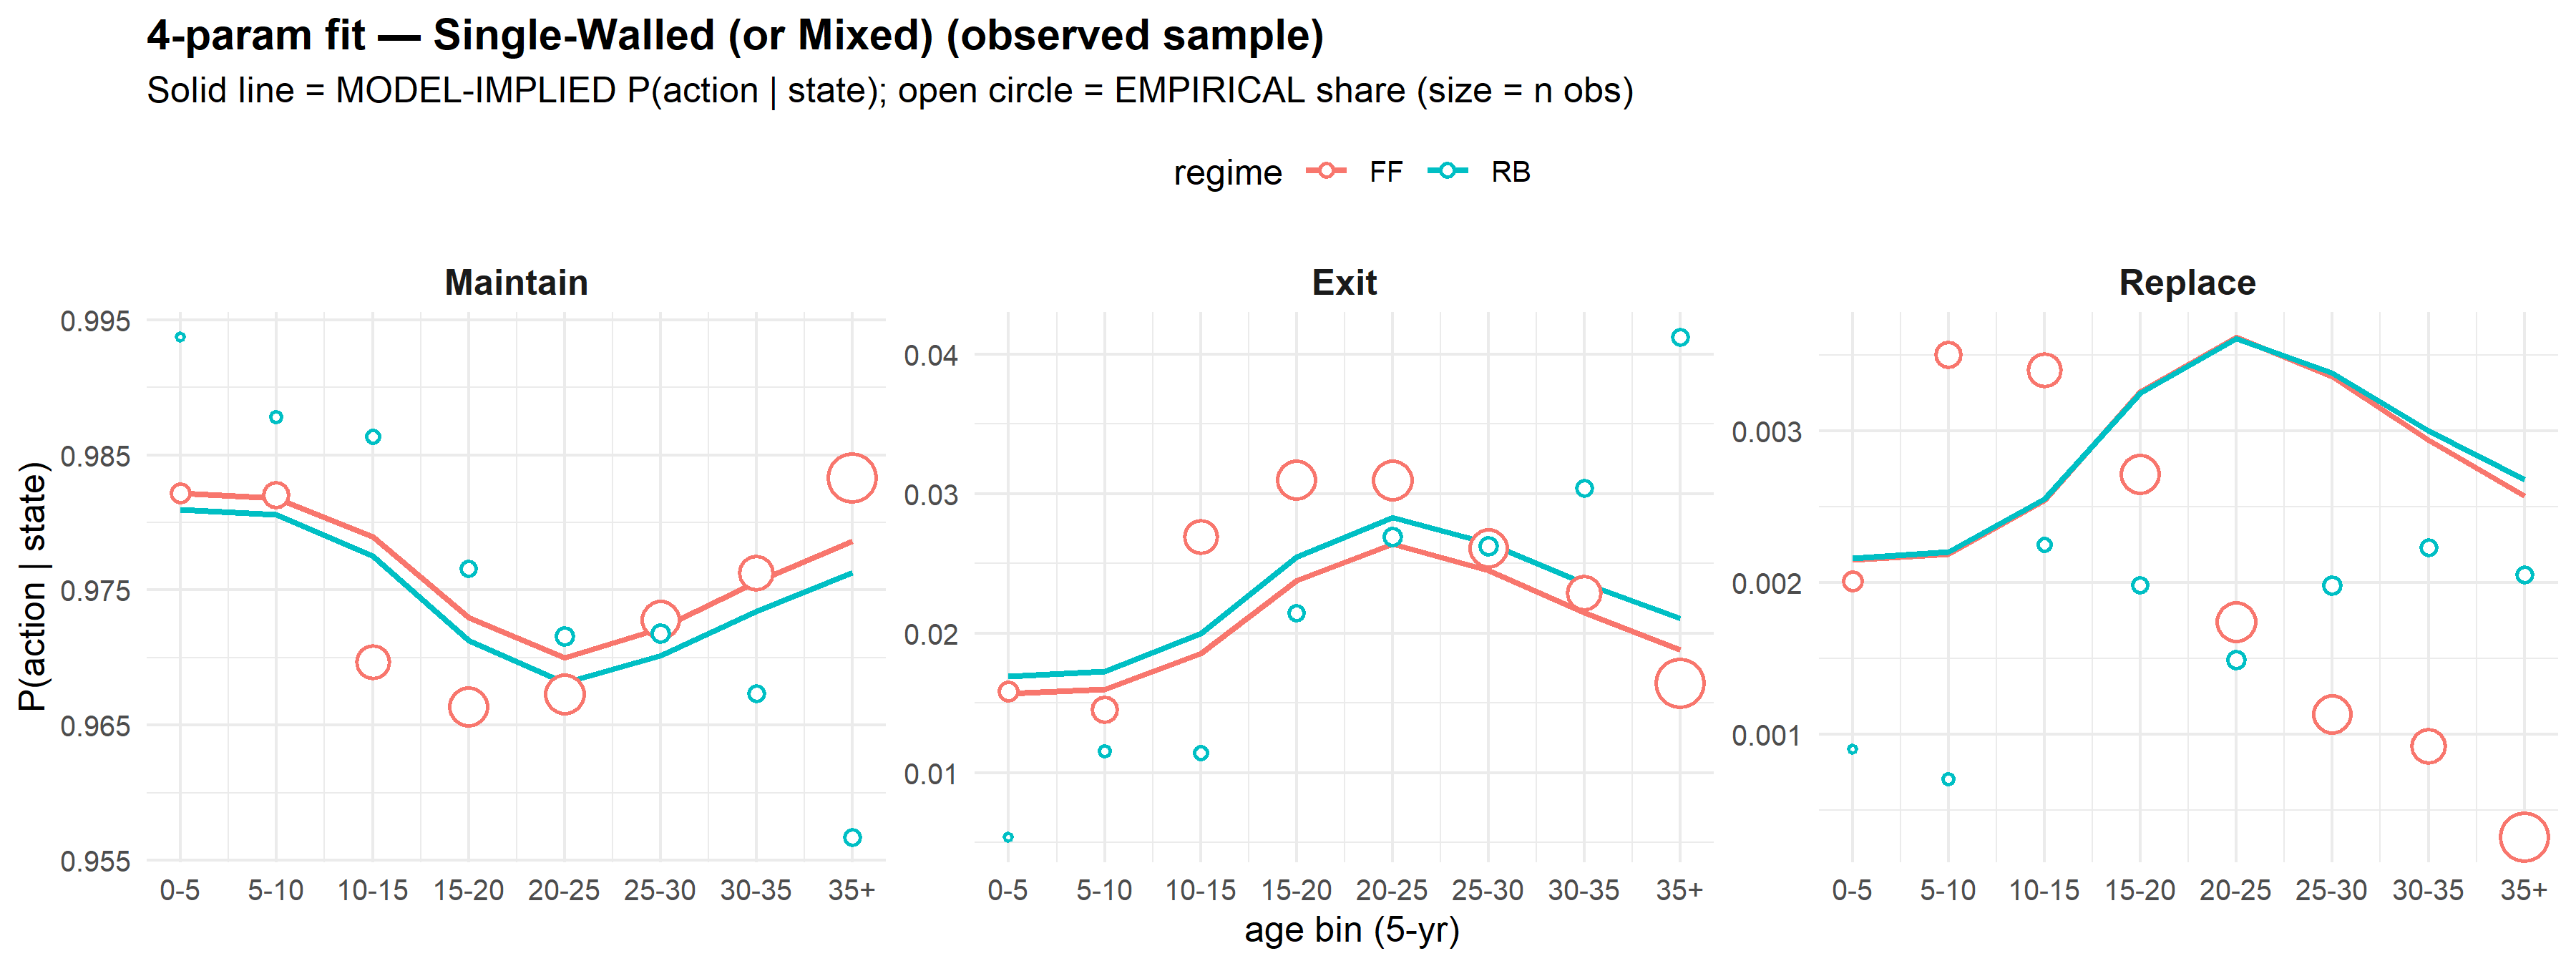
\includegraphics{../../Output/Figures/04k_Fit_4param_SW.png}

}

\end{figure}%

\begin{figure}[H]

\caption{\label{fig-fit-4p-dw}4-parameter fit, Double-Walled tanks. Same
construction as Figure~\ref{fig-fit-4p-sw}.}

\centering{

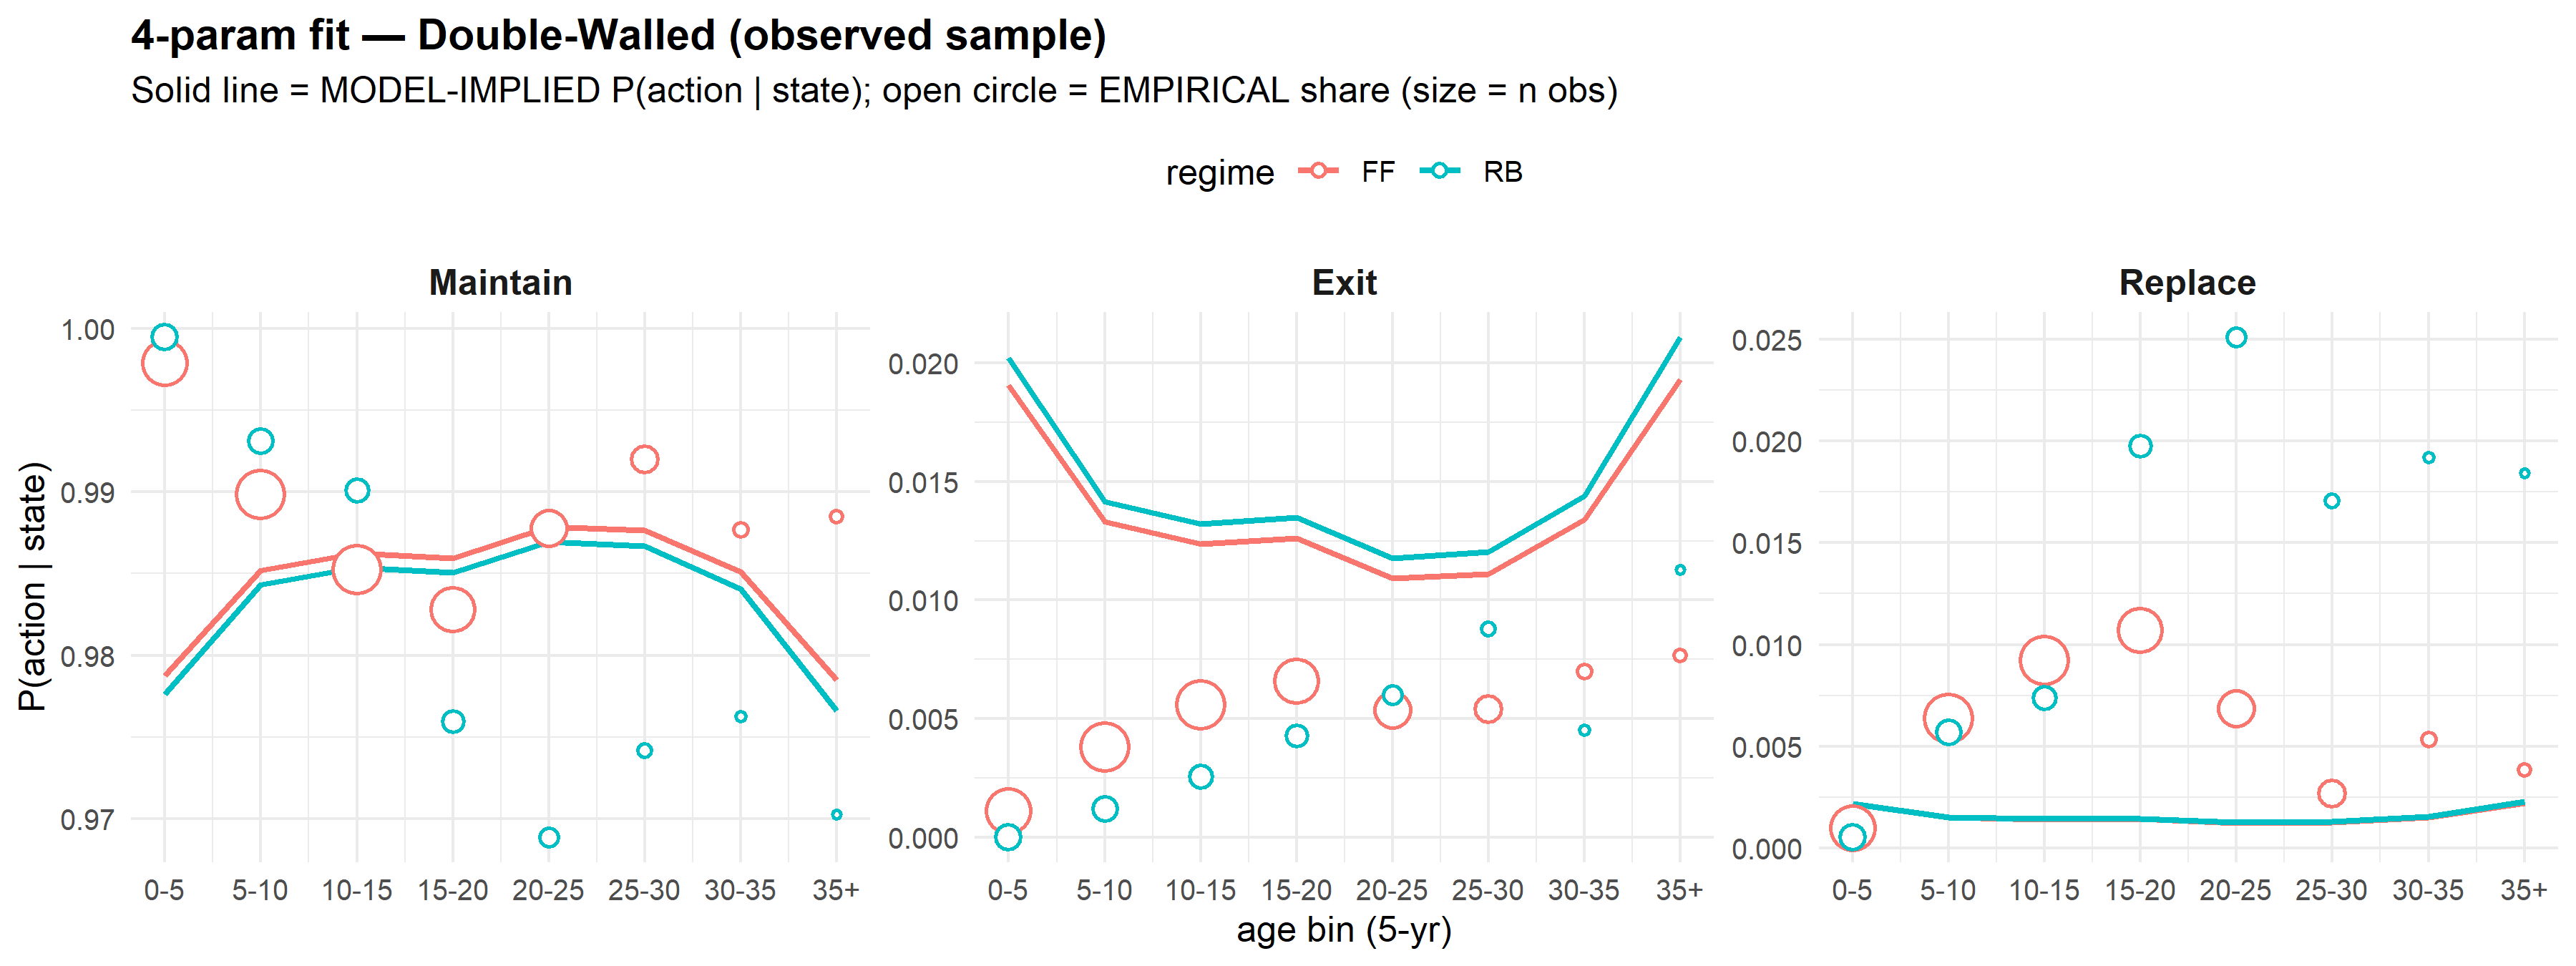
\includegraphics{../../Output/Figures/04k_Fit_4param_DW.png}

}

\end{figure}%

\begin{table}

\caption{\label{tbl-fitq-4p}4-parameter weighted-RMSE summary of
model-vs-empirical residuals by wall, regime, and action. Residual \(=\)
empirical \(-\) model share; weights are cell sample size.}

\centering{

\centering\begingroup\fontsize{9}{11}\selectfont

\resizebox{\ifdim\width>\linewidth\linewidth\else\width\fi}{!}{
\begin{tabular}{lllrrrrrrr}
\toprule
wall & regime & action & N\_cells & total\_n & unweighted\_mean\_residual & weighted\_mean\_residual & unweighted\_RMSE & weighted\_RMSE & max\_abs\_residual\\
\midrule
DW & FF & Exit & 8 & 351597 & -0.00870 & -0.00913 & 0.00959 & 0.01014 & 0.01795\\
DW & RB & Exit & 8 & 78616 & -0.01022 & -0.01222 & 0.01125 & 0.01326 & 0.02022\\
SW & FF & Exit & 8 & 1656628 & 0.00242 & 0.00237 & 0.00441 & 0.00453 & 0.00839\\
SW & RB & Exit & 8 & 195894 & -0.00055 & 0.00212 & 0.00943 & 0.00923 & 0.02020\\
DW & FF & Maintain & 8 & 351597 & 0.00456 & 0.00411 & 0.00809 & 0.00872 & 0.01913\\
\addlinespace
DW & RB & Maintain & 8 & 78616 & -0.00231 & 0.00351 & 0.01247 & 0.01396 & 0.02186\\
SW & FF & Maintain & 8 & 1656628 & -0.00156 & -0.00106 & 0.00446 & 0.00472 & 0.00924\\
SW & RB & Maintain & 8 & 195894 & 0.00170 & -0.00093 & 0.00972 & 0.00926 & 0.01957\\
DW & FF & Replace & 8 & 351597 & 0.00414 & 0.00502 & 0.00526 & 0.00616 & 0.00923\\
DW & RB & Replace & 8 & 78616 & 0.01253 & 0.00871 & 0.01493 & 0.01238 & 0.02386\\
\addlinespace
SW & FF & Replace & 8 & 1656628 & -0.00086 & -0.00131 & 0.00160 & 0.00179 & 0.00225\\
SW & RB & Replace & 8 & 195894 & -0.00116 & -0.00119 & 0.00127 & 0.00132 & 0.00212\\
\bottomrule
\end{tabular}}
\endgroup{}

}

\end{table}%

\subsection{8-parameter fit}\label{sec-fit-8p}

\begin{figure}[H]

\caption{\label{fig-fit-8p-sw}8-parameter fit, Single-Walled tanks. Same
construction as Figure~\ref{fig-fit-4p-sw}.}

\centering{

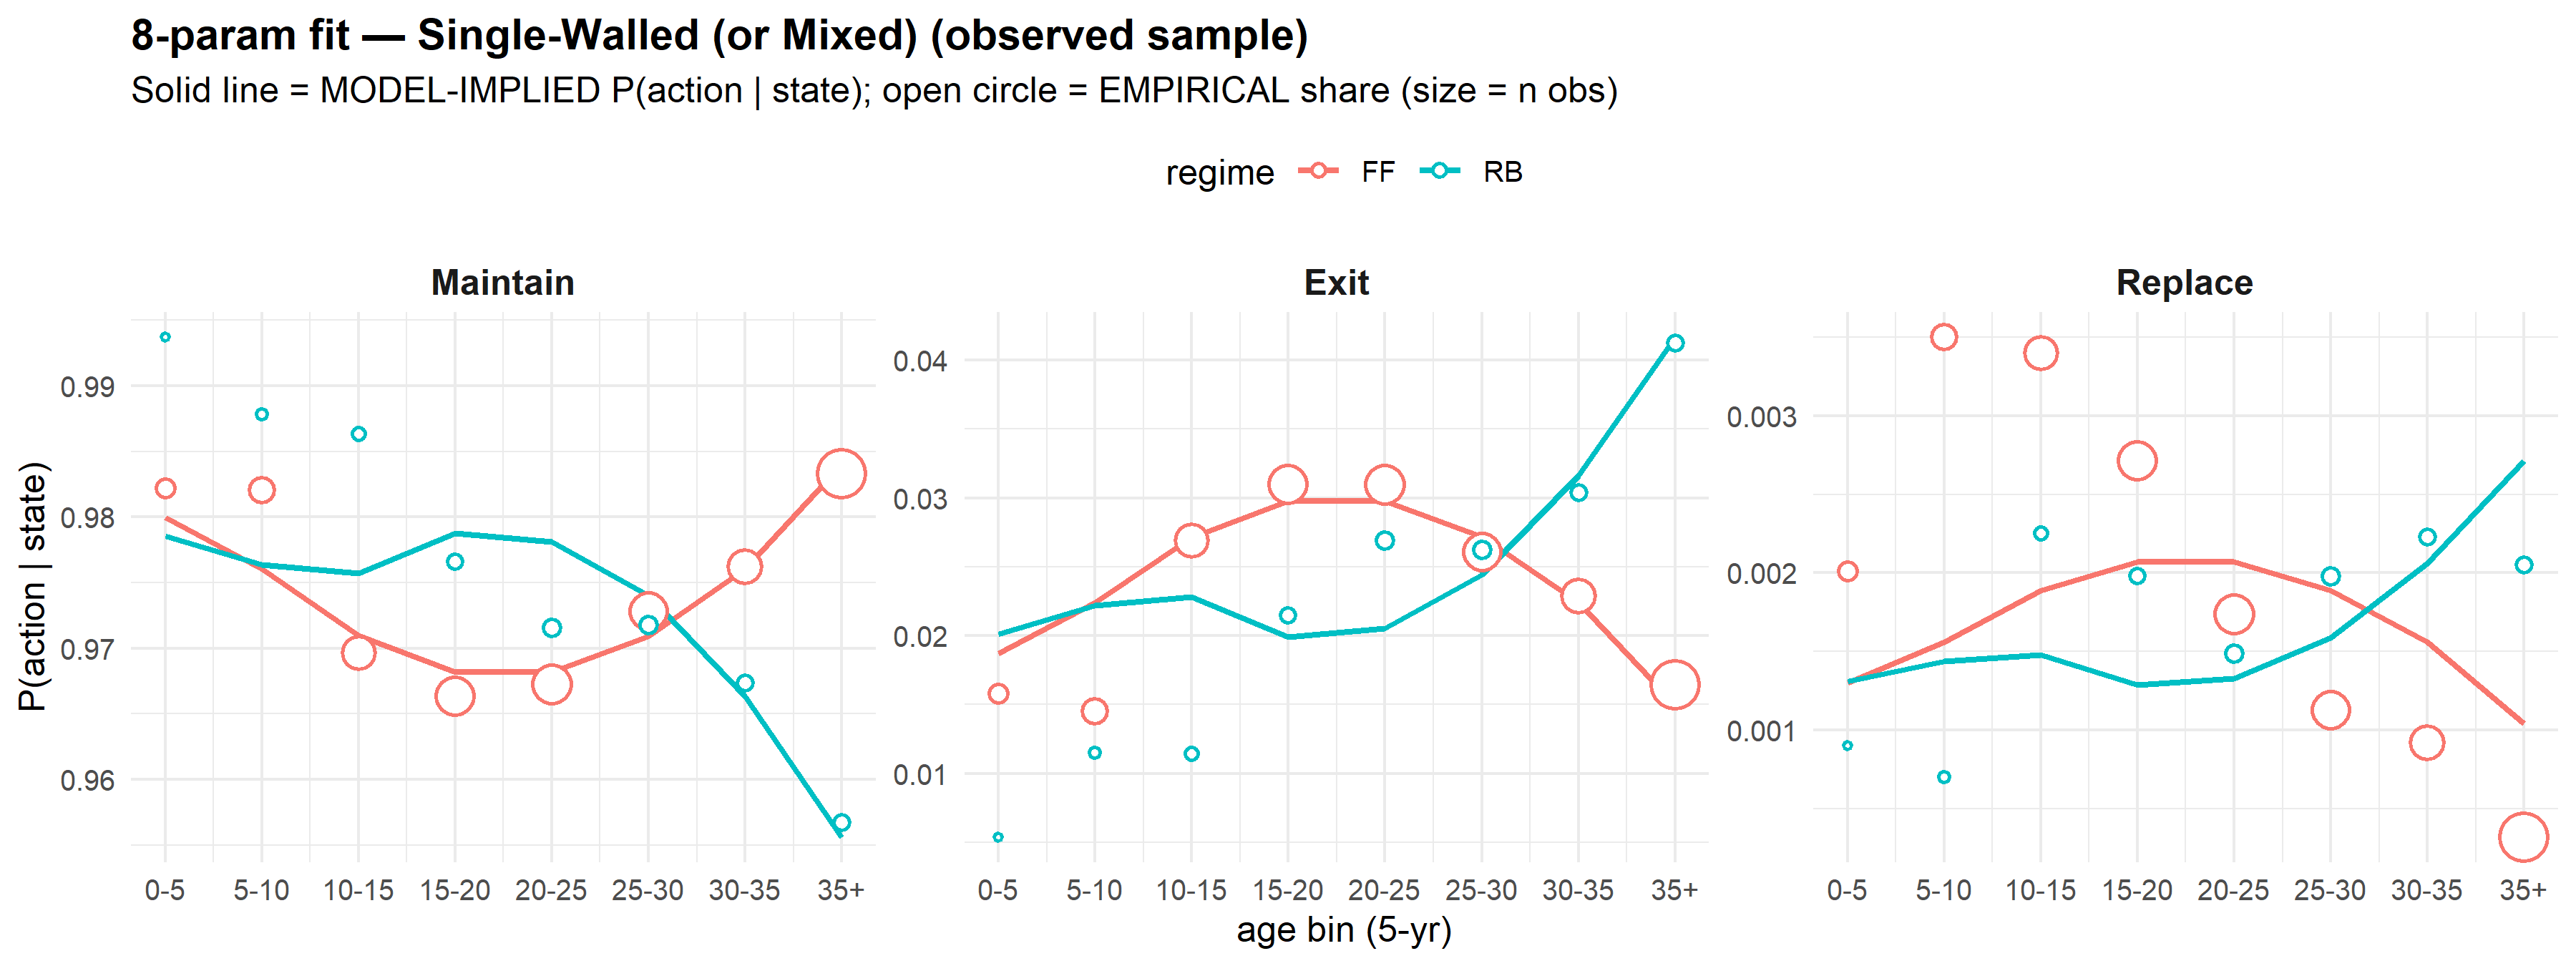
\includegraphics{../../Output/Figures/04k_Fit_8param_SW.png}

}

\end{figure}%

\begin{figure}[H]

\caption{\label{fig-fit-8p-dw}8-parameter fit, Double-Walled tanks. Same
construction as Figure~\ref{fig-fit-4p-sw}.}

\centering{

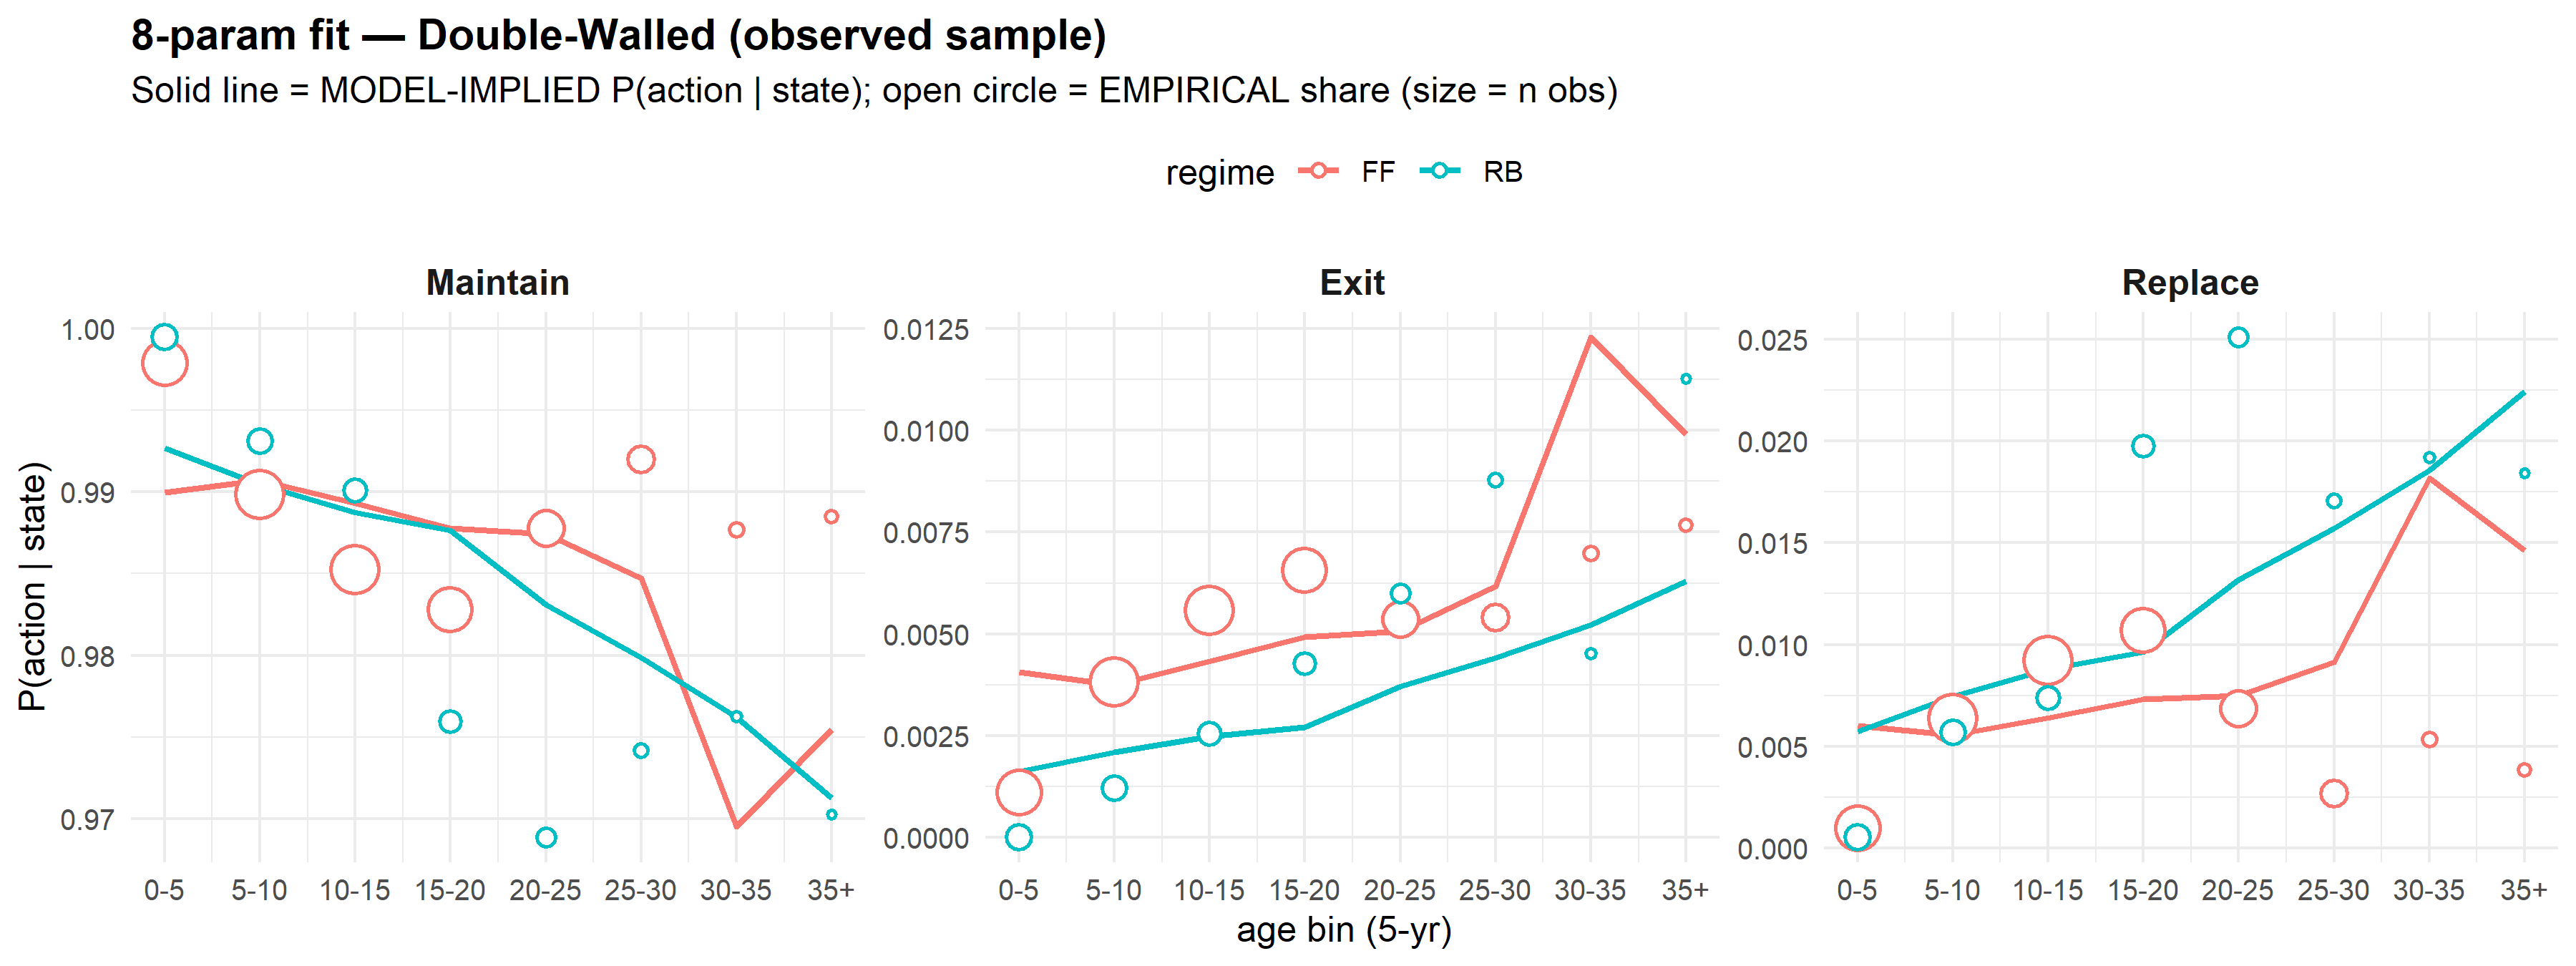
\includegraphics{../../Output/Figures/04k_Fit_8param_DW.png}

}

\end{figure}%

\begin{table}

\caption{\label{tbl-fitq-8p}8-parameter weighted-RMSE summary by wall,
regime, and action. Same construction as Table~\ref{tbl-fitq-4p}.}

\centering{

\centering\begingroup\fontsize{9}{11}\selectfont

\resizebox{\ifdim\width>\linewidth\linewidth\else\width\fi}{!}{
\begin{tabular}{lllrrrrr}
\toprule
wall & regime & action & N\_cells & total\_n & weighted\_RMSE & weighted\_mean\_residual & max\_abs\_residual\\
\midrule
DW & FF & Exit & 8 & 351597 & 0.00170 & -0.00006 & 0.00532\\
DW & RB & Exit & 8 & 78616 & 0.00176 & 0.00024 & 0.00497\\
SW & FF & Exit & 8 & 1656628 & 0.00227 & 0.00005 & 0.00792\\
SW & RB & Exit & 8 & 195894 & 0.00558 & -0.00042 & 0.01475\\
DW & FF & Maintain & 8 & 351597 & 0.00537 & 0.00031 & 0.01818\\
\addlinespace
DW & RB & Maintain & 8 & 78616 & 0.00773 & -0.00140 & 0.01421\\
SW & FF & Maintain & 8 & 1656628 & 0.00193 & -0.00003 & 0.00598\\
SW & RB & Maintain & 8 & 195894 & 0.00563 & 0.00027 & 0.01516\\
DW & FF & Replace & 8 & 351597 & 0.00378 & -0.00024 & 0.01286\\
DW & RB & Replace & 8 & 78616 & 0.00637 & 0.00117 & 0.01192\\
\addlinespace
SW & FF & Replace & 8 & 1656628 & 0.00090 & -0.00002 & 0.00194\\
SW & RB & Replace & 8 & 195894 & 0.00051 & 0.00015 & 0.00077\\
\bottomrule
\end{tabular}}
\endgroup{}

}

\end{table}%

\subsection{8-parameter + FE (M-only, joint) fit}\label{sec-fit-8pfe}

\begin{figure}[H]

\caption{\label{fig-fit-8pfe-sw}8-parameter + FE fit, Single-Walled
tanks. Model-implied probabilities marginalize the per-\(g\) choice
probability over the empirical state composition \(w_g(s)\). Same plot
construction as Figure~\ref{fig-fit-4p-sw}.}

\centering{

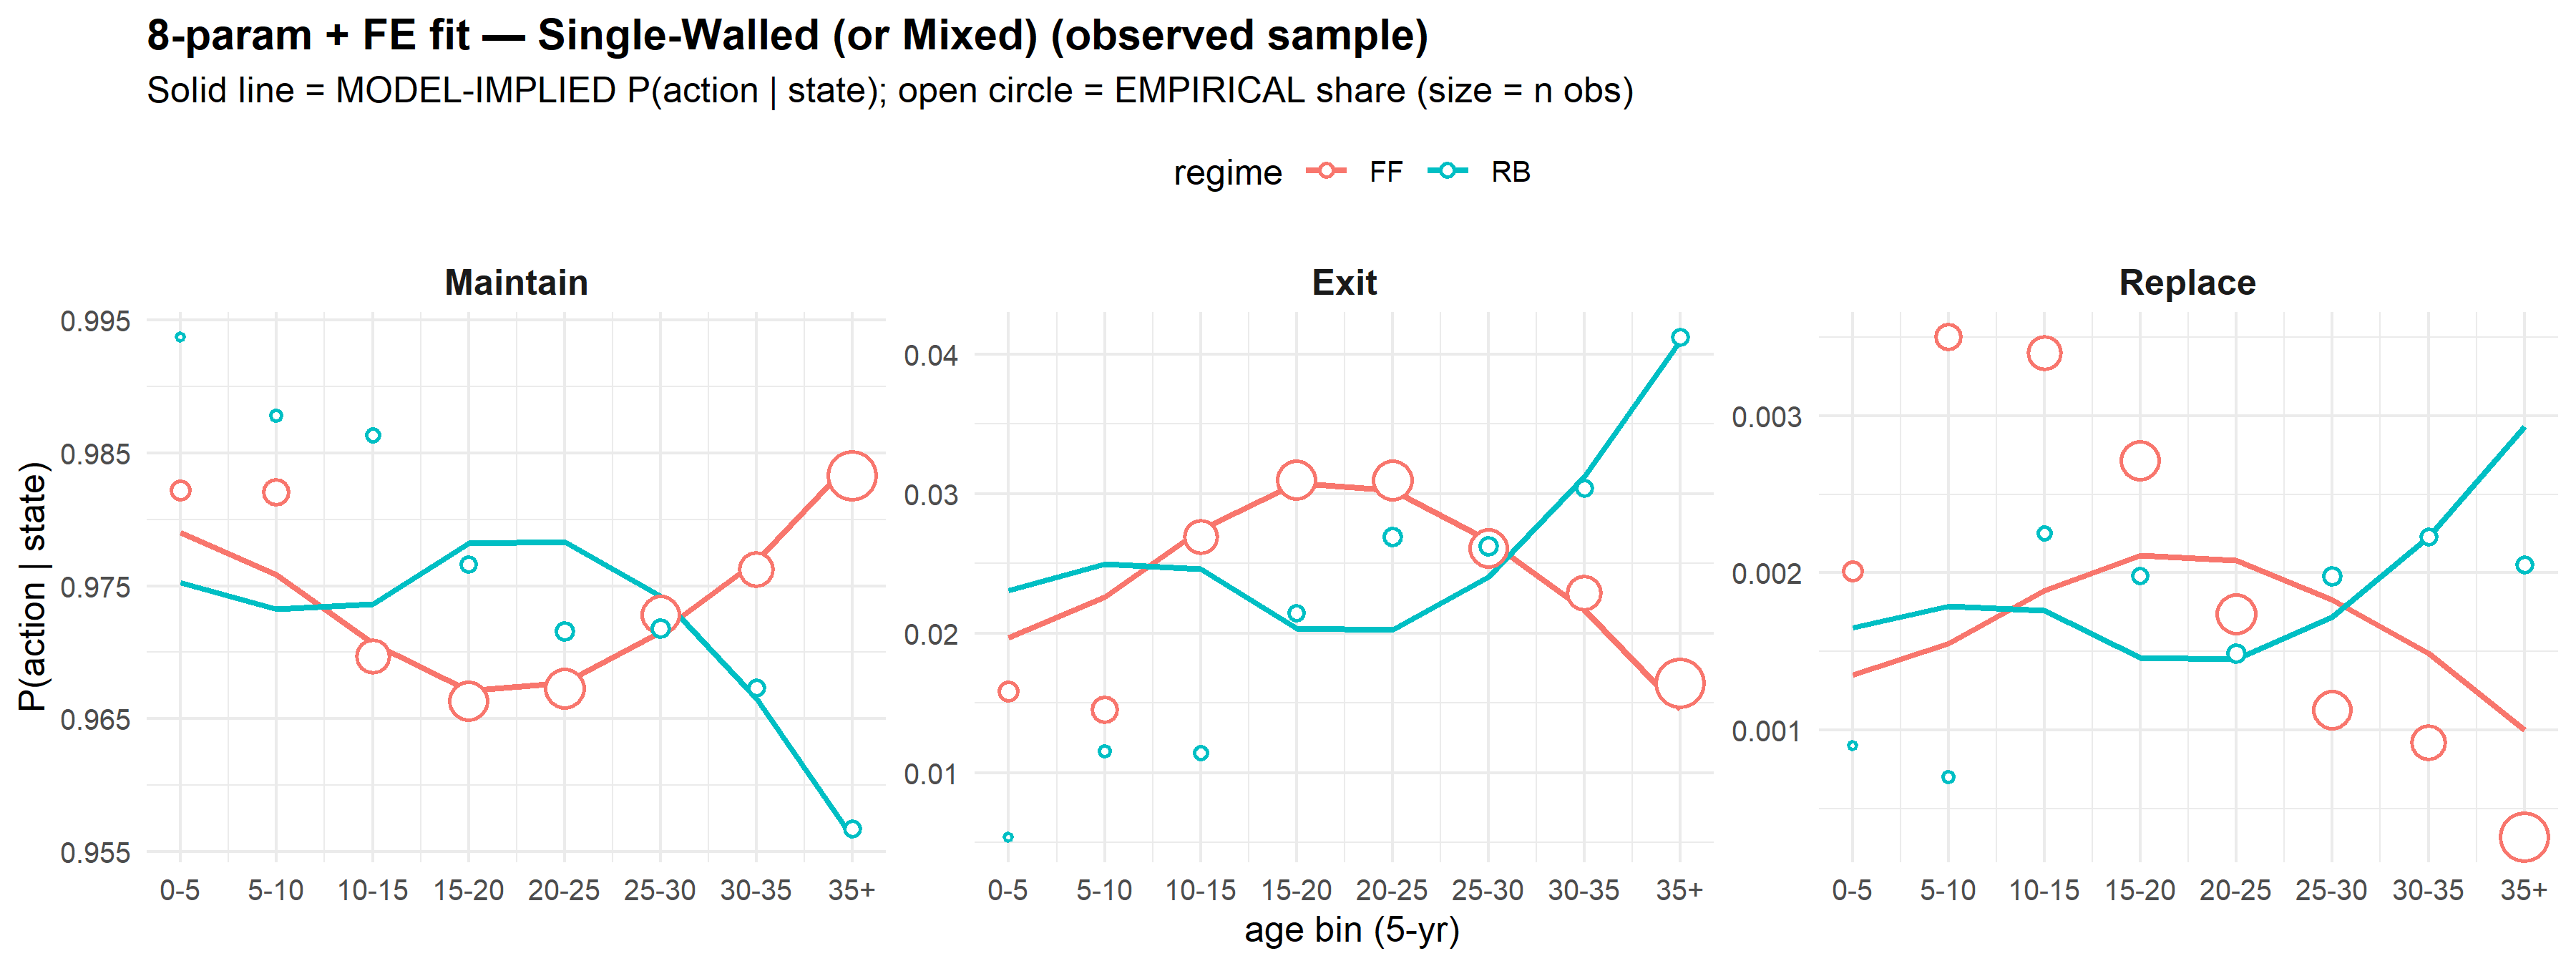
\includegraphics{../../Output/Figures/04k_Fit_8paramFE_SW.png}

}

\end{figure}%

\begin{figure}[H]

\caption{\label{fig-fit-8pfe-dw}8-parameter + FE fit, Double-Walled
tanks. Same construction as Figure~\ref{fig-fit-8pfe-sw}.}

\centering{

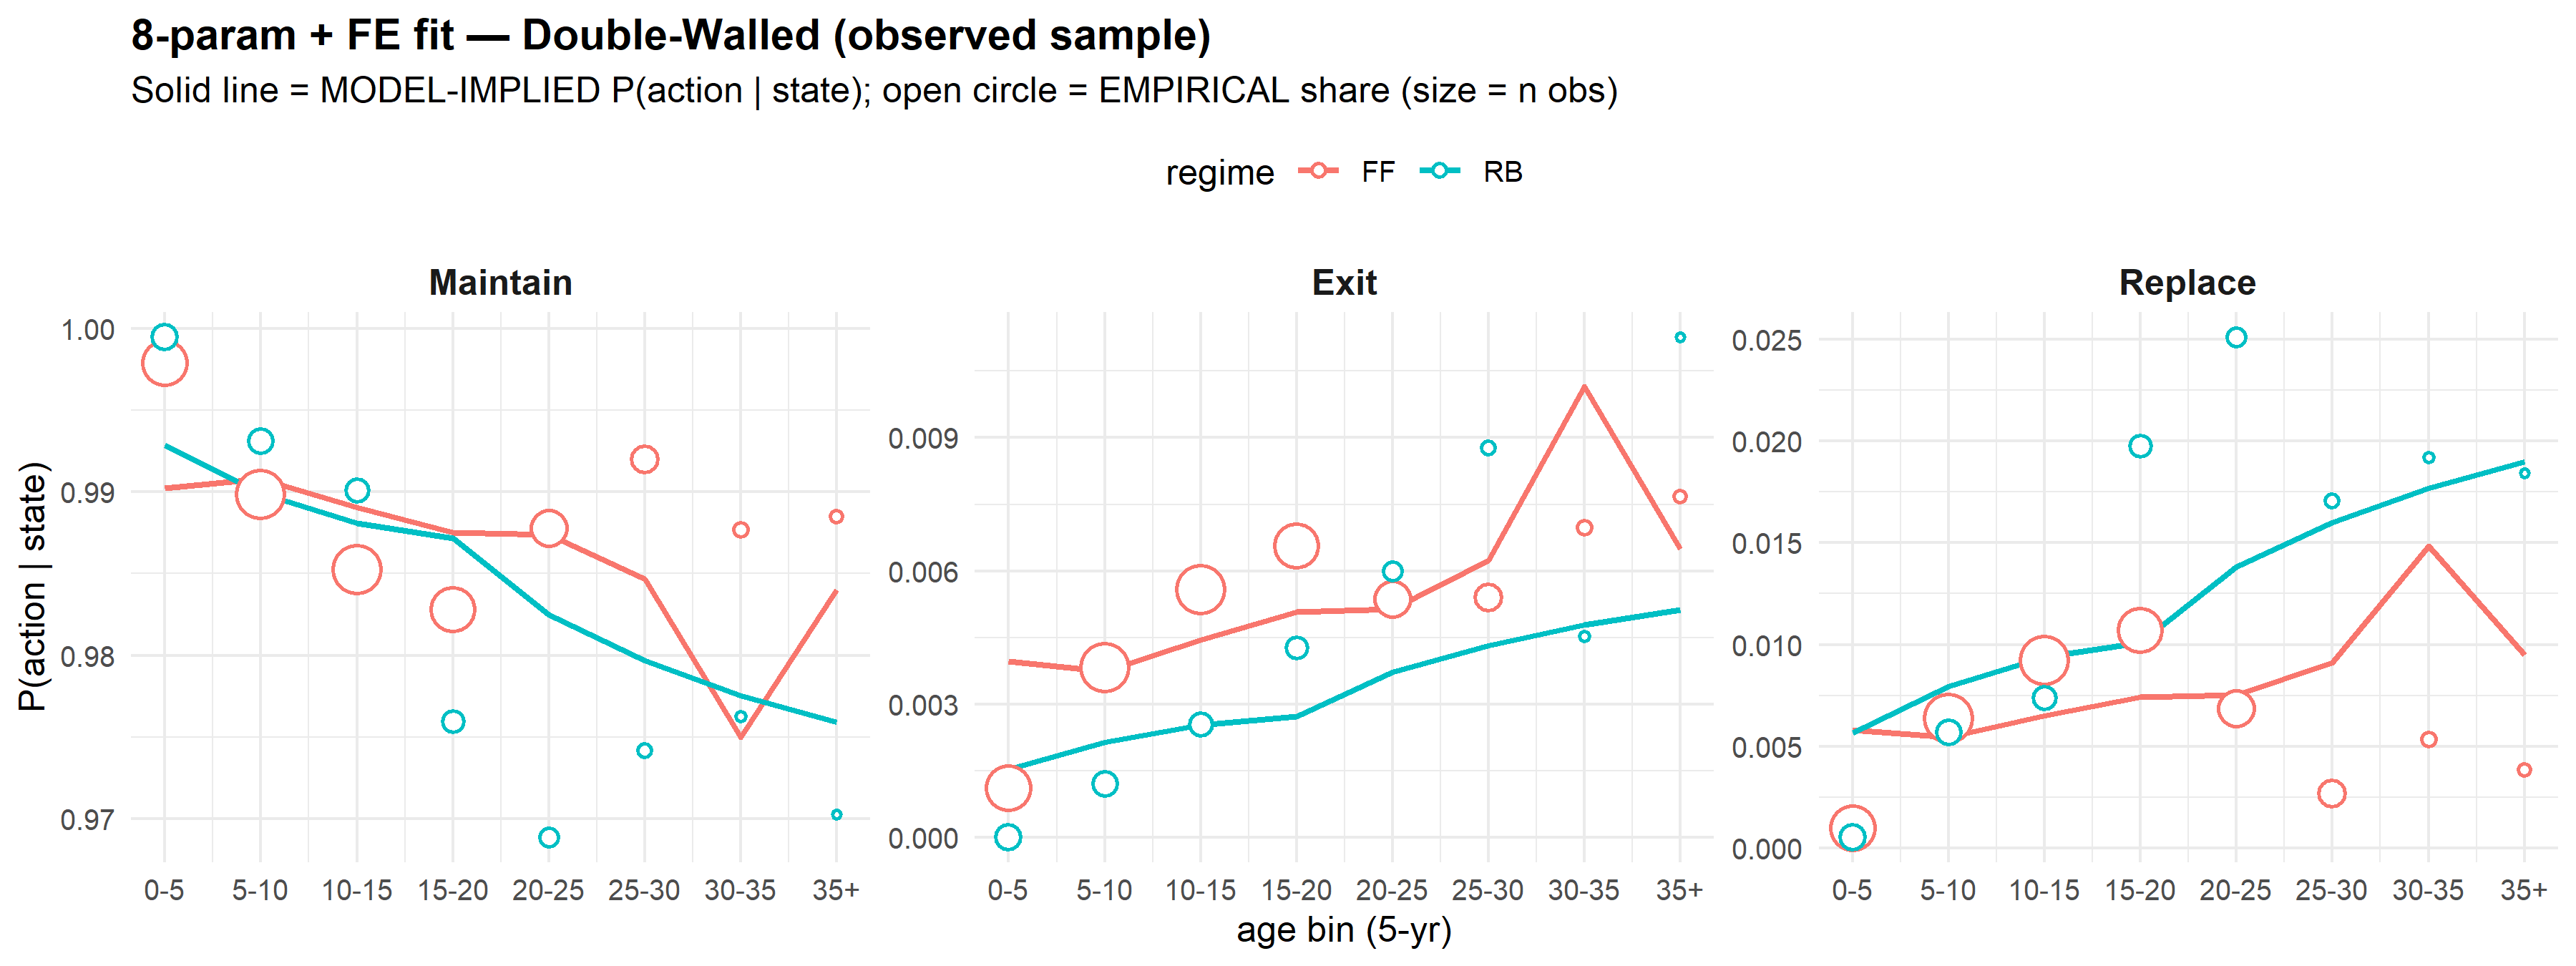
\includegraphics{../../Output/Figures/04k_Fit_8paramFE_DW.png}

}

\end{figure}%

\begin{table}

\caption{\label{tbl-fitq-8pfe}8-parameter + FE (M-only, joint)
weighted-RMSE summary by wall, regime, and action. Same construction as
Table~\ref{tbl-fitq-4p}.}

\centering{

\centering\begingroup\fontsize{9}{11}\selectfont

\resizebox{\ifdim\width>\linewidth\linewidth\else\width\fi}{!}{
\begin{tabular}{lllrrrrr}
\toprule
wall & regime & action & N\_cells & total\_n & weighted\_RMSE & weighted\_mean\_residual & max\_abs\_residual\\
\midrule
DW & FF & Exit & 8 & 351597 & 0.00154 & -0.00005 & 0.00317\\
DW & RB & Exit & 8 & 78616 & 0.00180 & 0.00026 & 0.00615\\
SW & FF & Exit & 8 & 1656628 & 0.00235 & 0.00002 & 0.00810\\
SW & RB & Exit & 8 & 195894 & 0.00642 & -0.00054 & 0.01771\\
DW & FF & Maintain & 8 & 351597 & 0.00486 & 0.00020 & 0.01267\\
\addlinespace
DW & RB & Maintain & 8 & 78616 & 0.00754 & -0.00114 & 0.01359\\
SW & FF & Maintain & 8 & 1656628 & 0.00184 & -0.00003 & 0.00616\\
SW & RB & Maintain & 8 & 195894 & 0.00652 & 0.00057 & 0.01846\\
DW & FF & Replace & 8 & 351597 & 0.00345 & -0.00015 & 0.00950\\
DW & RB & Replace & 8 & 78616 & 0.00616 & 0.00088 & 0.01132\\
\addlinespace
SW & FF & Replace & 8 & 1656628 & 0.00088 & 0.00000 & 0.00195\\
SW & RB & Replace & 8 & 195894 & 0.00052 & -0.00003 & 0.00109\\
\bottomrule
\end{tabular}}
\endgroup{}

}

\end{table}%

\subsection{8-parameter + stayFE (profile)
fit}\label{sec-fit-8pfeProfile}

\begin{figure}[H]

\caption{\label{fig-fit-8pfeProfile-sw}8-parameter + stayFE (profile)
fit, Single-Walled tanks. Same construction as
Figure~\ref{fig-fit-4p-sw}. Model-implied probabilities marginalize the
per-\(g\) choice probability over the empirical state composition
\(w_g(s)\), with \(\alpha_g\) entering both Maintain and Replace
utilities (profiled out via 1-D FOC).}

\centering{

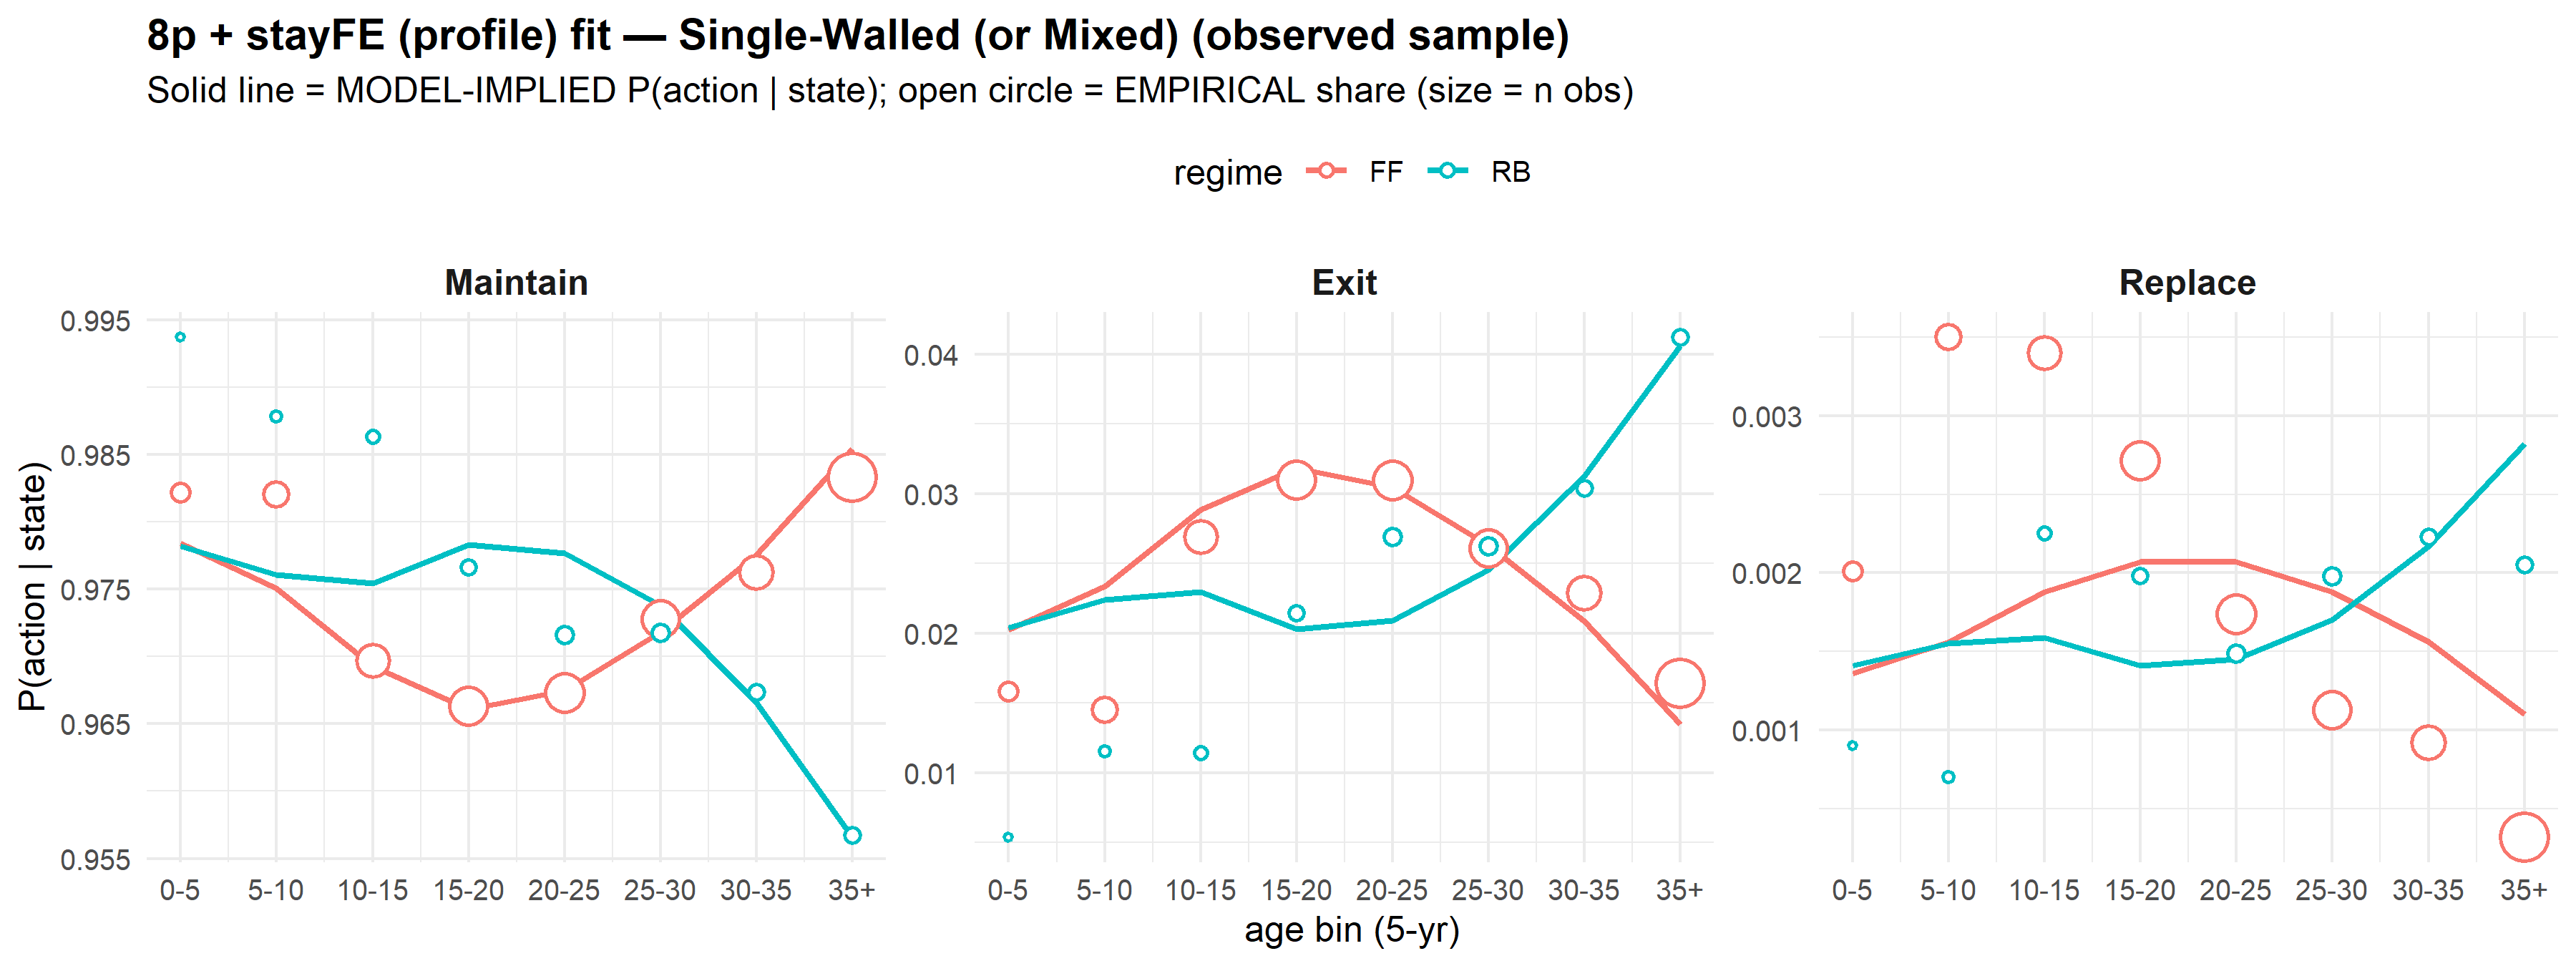
\includegraphics{../../Output/Figures/04l_Fit_8paramFE_profile_SW.png}

}

\end{figure}%

\begin{figure}[H]

\caption{\label{fig-fit-8pfeProfile-dw}8-parameter + stayFE (profile)
fit, Double-Walled tanks. Same construction as
Figure~\ref{fig-fit-8pfeProfile-sw}.}

\centering{

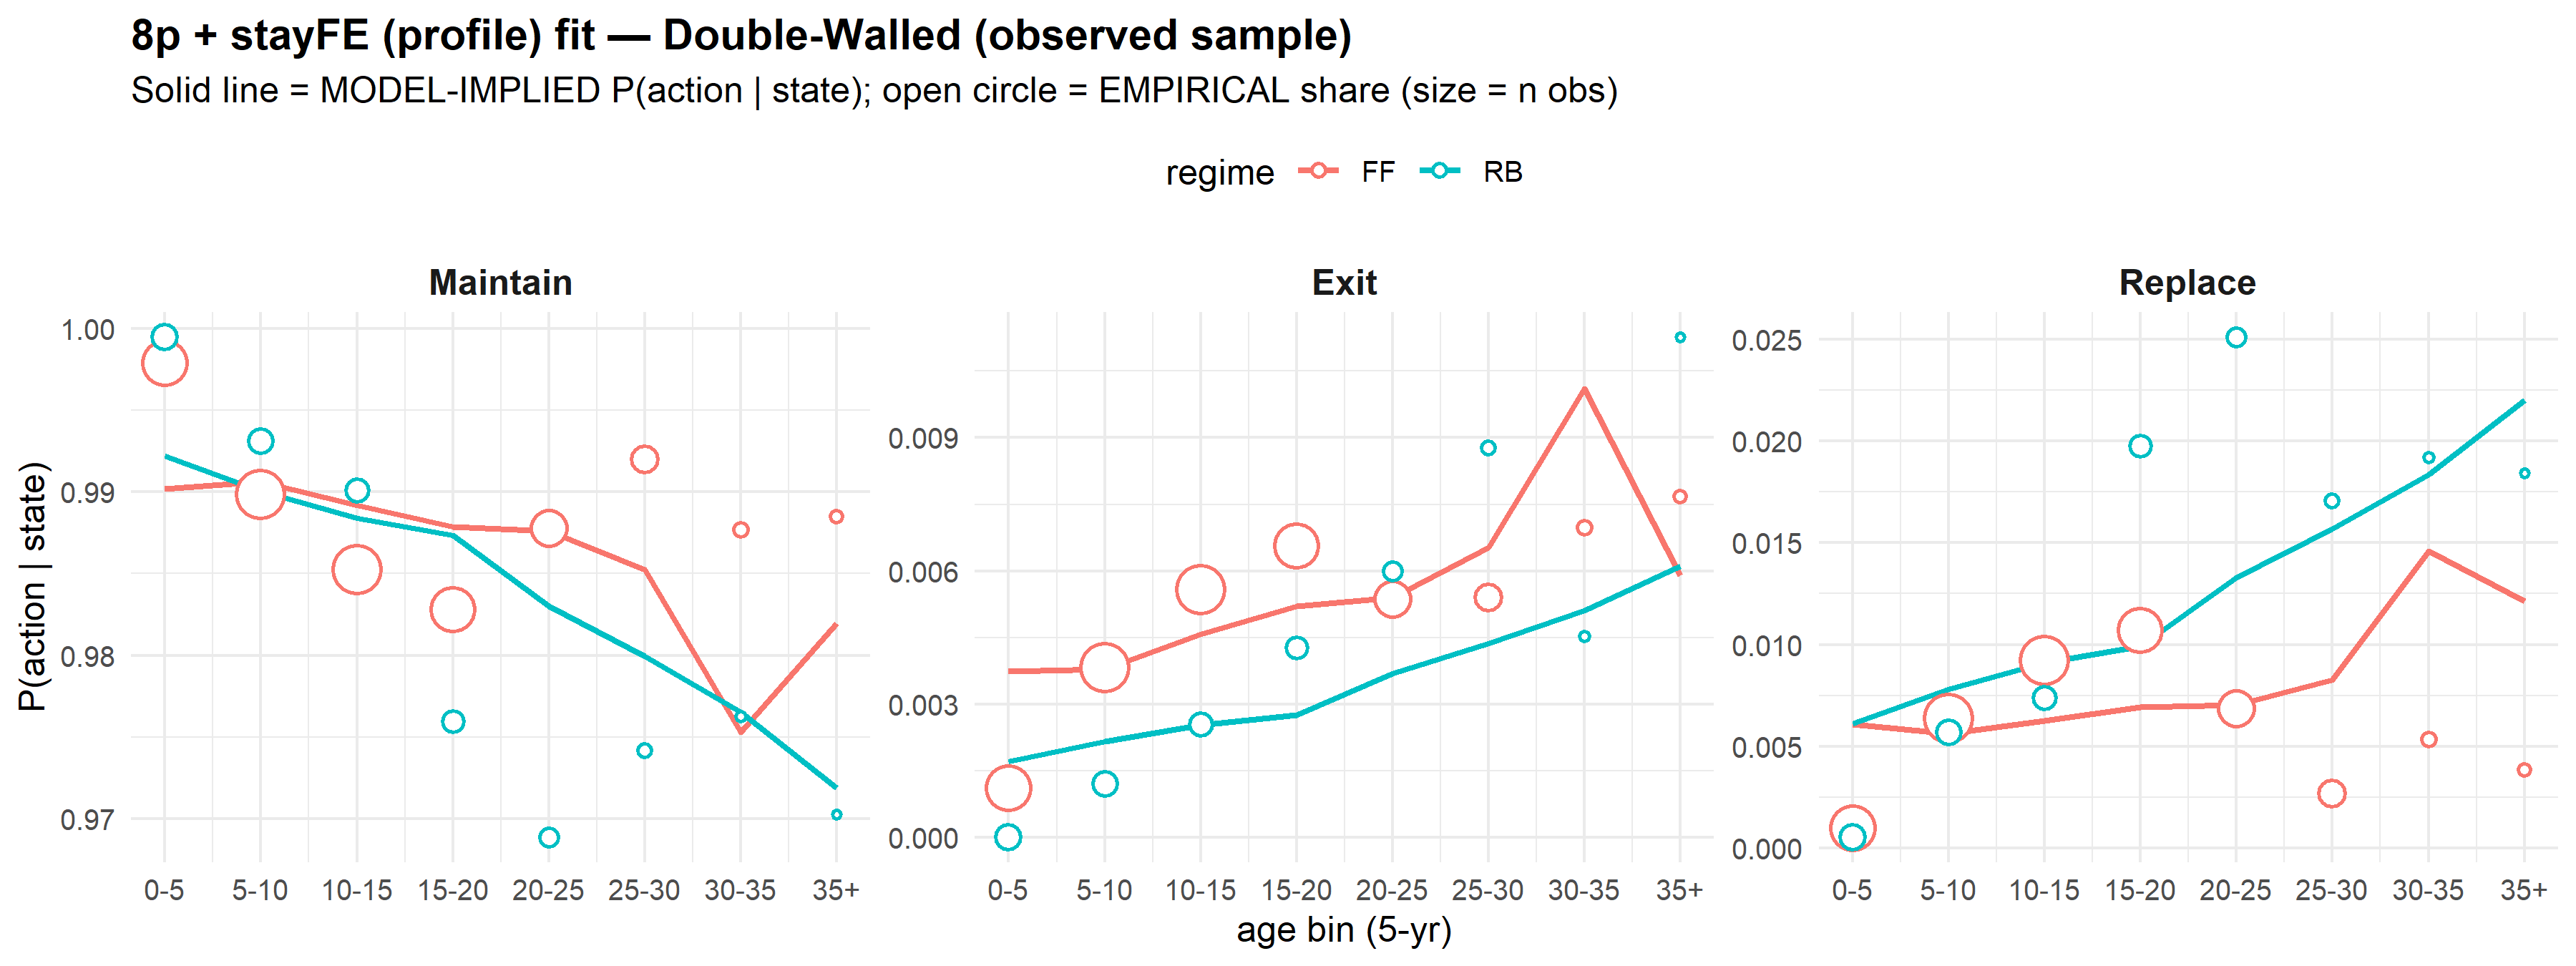
\includegraphics{../../Output/Figures/04l_Fit_8paramFE_profile_DW.png}

}

\end{figure}%

\begin{table}

\caption{\label{tbl-fitq-8pfeProfile}8-parameter + stayFE (profile)
weighted-RMSE summary by wall, regime, and action. Same construction as
Table~\ref{tbl-fitq-4p}.}

\centering{

\centering\begingroup\fontsize{9}{11}\selectfont

\resizebox{\ifdim\width>\linewidth\linewidth\else\width\fi}{!}{
\begin{tabular}{lllrrrrr}
\toprule
wall & regime & action & N\_cells & total\_n & weighted\_RMSE & weighted\_mean\_residual & max\_abs\_residual\\
\midrule
DW & FF & Exit & 8 & 351597 & 0.00143 & -0.00011 & 0.00313\\
DW & RB & Exit & 8 & 78616 & 0.00180 & 0.00019 & 0.00516\\
SW & FF & Exit & 8 & 1656628 & 0.00290 & 0.00002 & 0.00889\\
SW & RB & Exit & 8 & 195894 & 0.00554 & -0.00036 & 0.01503\\
DW & FF & Maintain & 8 & 351597 & 0.00492 & 0.00011 & 0.01239\\
\addlinespace
DW & RB & Maintain & 8 & 78616 & 0.00778 & -0.00109 & 0.01412\\
SW & FF & Maintain & 8 & 1656628 & 0.00219 & 0.00001 & 0.00695\\
SW & RB & Maintain & 8 & 195894 & 0.00557 & 0.00032 & 0.01555\\
DW & FF & Replace & 8 & 351597 & 0.00359 & 0.00000 & 0.00926\\
DW & RB & Replace & 8 & 78616 & 0.00639 & 0.00090 & 0.01182\\
\addlinespace
SW & FF & Replace & 8 & 1656628 & 0.00092 & -0.00003 & 0.00194\\
SW & RB & Replace & 8 & 195894 & 0.00049 & 0.00004 & 0.00085\\
\bottomrule
\end{tabular}}
\endgroup{}

}

\end{table}%

\section{Appendix: Per-cell fit numbers}\label{sec-appendix}

The following three tables report the full 32-row cell-level fit numbers
for each specification. Columns: \texttt{Reg} (regime: FF/RB),
\texttt{Wall} (SW/DW), \texttt{Age} (5-year bin), \texttt{N} (cell
sample size), and for each of the three actions \(a \in \{M, E, R\}\),
\texttt{mod\_a} \(= \hat P_a(s)\) (model-implied), \texttt{emp\_a}
(empirical share), and \texttt{res\_a} \(=\) \texttt{emp\_a} \(-\)
\texttt{mod\_a} (residual).

\subsection{4-parameter}\label{sec-appendix-4p}

\begingroup\fontsize{8}{10}\selectfont

\begin{longtable}{lllrrrrrrrrrr}

\caption{\label{tbl-appendix-4p}4-parameter per-cell fit: model-implied
probability, empirical share, and residual by state cell.}

\tabularnewline

\toprule
Reg & Wall & Age & N & mod\_M & emp\_M & res\_M & mod\_E & emp\_E & res\_E & mod\_R & emp\_R & res\_R\\
\midrule
FF & DW & 0-5 & 64621 & 0.9788 & 0.9979 & 0.0191 & 0.0191 & 0.0011 & -0.0180 & 0.0022 & 0.0010 & -0.0012\\
FF & DW & 5-10 & 77103 & 0.9852 & 0.9898 & 0.0046 & 0.0133 & 0.0038 & -0.0095 & 0.0015 & 0.0064 & 0.0048\\
FF & DW & 10-15 & 77966 & 0.9862 & 0.9852 & -0.0010 & 0.0124 & 0.0056 & -0.0068 & 0.0014 & 0.0092 & 0.0078\\
FF & DW & 15-20 & 62241 & 0.9860 & 0.9828 & -0.0032 & 0.0126 & 0.0066 & -0.0061 & 0.0014 & 0.0107 & 0.0092\\
FF & DW & 20-25 & 41520 & 0.9878 & 0.9878 & -0.0001 & 0.0109 & 0.0054 & -0.0055 & 0.0012 & 0.0069 & 0.0056\\
\addlinespace
FF & DW & 25-30 & 20407 & 0.9876 & 0.9920 & 0.0043 & 0.0111 & 0.0054 & -0.0057 & 0.0013 & 0.0026 & 0.0014\\
FF & DW & 30-35 & 4872 & 0.9851 & 0.9877 & 0.0026 & 0.0134 & 0.0070 & -0.0064 & 0.0015 & 0.0053 & 0.0038\\
FF & DW & 35+ & 2867 & 0.9785 & 0.9885 & 0.0100 & 0.0193 & 0.0077 & -0.0116 & 0.0022 & 0.0038 & 0.0016\\
FF & SW & 0-5 & 46709 & 0.9822 & 0.9822 & 0.0000 & 0.0157 & 0.0158 & 0.0001 & 0.0022 & 0.0020 & -0.0001\\
FF & SW & 5-10 & 97999 & 0.9818 & 0.9820 & 0.0002 & 0.0160 & 0.0145 & -0.0015 & 0.0022 & 0.0035 & 0.0013\\
\addlinespace
FF & SW & 10-15 & 180163 & 0.9789 & 0.9697 & -0.0092 & 0.0185 & 0.0269 & 0.0084 & 0.0025 & 0.0034 & 0.0009\\
FF & SW & 15-20 & 240344 & 0.9730 & 0.9663 & -0.0066 & 0.0238 & 0.0310 & 0.0072 & 0.0033 & 0.0027 & -0.0006\\
FF & SW & 20-25 & 255278 & 0.9700 & 0.9673 & -0.0027 & 0.0264 & 0.0310 & 0.0046 & 0.0036 & 0.0017 & -0.0019\\
FF & SW & 25-30 & 234030 & 0.9722 & 0.9728 & 0.0006 & 0.0245 & 0.0261 & 0.0016 & 0.0034 & 0.0011 & -0.0022\\
FF & SW & 30-35 & 191377 & 0.9756 & 0.9762 & 0.0006 & 0.0215 & 0.0228 & 0.0014 & 0.0029 & 0.0009 & -0.0020\\
\addlinespace
FF & SW & 35+ & 410728 & 0.9786 & 0.9833 & 0.0046 & 0.0188 & 0.0164 & -0.0024 & 0.0026 & 0.0003 & -0.0022\\
RB & DW & 0-5 & 18813 & 0.9776 & 0.9995 & 0.0219 & 0.0202 & 0.0000 & -0.0202 & 0.0022 & 0.0005 & -0.0016\\
RB & DW & 5-10 & 16557 & 0.9843 & 0.9931 & 0.0088 & 0.0142 & 0.0012 & -0.0130 & 0.0015 & 0.0057 & 0.0042\\
RB & DW & 10-15 & 14499 & 0.9854 & 0.9901 & 0.0047 & 0.0132 & 0.0026 & -0.0106 & 0.0014 & 0.0074 & 0.0060\\
RB & DW & 15-20 & 13106 & 0.9851 & 0.9760 & -0.0091 & 0.0135 & 0.0043 & -0.0092 & 0.0014 & 0.0198 & 0.0183\\
\addlinespace
RB & DW & 20-25 & 8677 & 0.9870 & 0.9689 & -0.0181 & 0.0118 & 0.0060 & -0.0058 & 0.0013 & 0.0251 & 0.0239\\
RB & DW & 25-30 & 4218 & 0.9867 & 0.9742 & -0.0125 & 0.0120 & 0.0088 & -0.0033 & 0.0013 & 0.0171 & 0.0158\\
RB & DW & 30-35 & 1770 & 0.9841 & 0.9763 & -0.0078 & 0.0144 & 0.0045 & -0.0099 & 0.0015 & 0.0192 & 0.0177\\
RB & DW & 35+ & 976 & 0.9766 & 0.9703 & -0.0063 & 0.0211 & 0.0113 & -0.0098 & 0.0023 & 0.0184 & 0.0162\\
RB & SW & 0-5 & 3350 & 0.9810 & 0.9937 & 0.0128 & 0.0169 & 0.0054 & -0.0115 & 0.0022 & 0.0009 & -0.0013\\
\addlinespace
RB & SW & 5-10 & 9999 & 0.9806 & 0.9878 & 0.0072 & 0.0172 & 0.0115 & -0.0057 & 0.0022 & 0.0007 & -0.0015\\
RB & SW & 10-15 & 19093 & 0.9775 & 0.9863 & 0.0088 & 0.0200 & 0.0114 & -0.0085 & 0.0026 & 0.0022 & -0.0003\\
RB & SW & 15-20 & 26212 & 0.9713 & 0.9766 & 0.0053 & 0.0255 & 0.0214 & -0.0040 & 0.0032 & 0.0020 & -0.0013\\
RB & SW & 20-25 & 36841 & 0.9681 & 0.9716 & 0.0035 & 0.0283 & 0.0269 & -0.0014 & 0.0036 & 0.0015 & -0.0021\\
RB & SW & 25-30 & 37789 & 0.9702 & 0.9718 & 0.0016 & 0.0265 & 0.0262 & -0.0003 & 0.0034 & 0.0020 & -0.0014\\
\addlinespace
RB & SW & 30-35 & 31888 & 0.9734 & 0.9674 & -0.0061 & 0.0236 & 0.0304 & 0.0069 & 0.0030 & 0.0022 & -0.0008\\
RB & SW & 35+ & 30722 & 0.9763 & 0.9567 & -0.0196 & 0.0210 & 0.0412 & 0.0202 & 0.0027 & 0.0021 & -0.0006\\
\bottomrule

\end{longtable}

\endgroup{}

\subsection{8-parameter}\label{sec-appendix-8p}

\begingroup\fontsize{8}{10}\selectfont

\begin{longtable}{lllrrrrrrrrrr}

\caption{\label{tbl-appendix-8p}8-parameter per-cell fit. Same
construction as Table~\ref{tbl-appendix-4p}.}

\tabularnewline

\toprule
Reg & Wall & Age & N & mod\_M & emp\_M & res\_M & mod\_E & emp\_E & res\_E & mod\_R & emp\_R & res\_R\\
\midrule
FF & DW & 0-5 & 64621 & 0.9899 & 0.9979 & 0.0080 & 0.0041 & 0.0011 & -0.0029 & 0.0060 & 0.0010 & -0.0050\\
FF & DW & 5-10 & 77103 & 0.9907 & 0.9898 & -0.0009 & 0.0037 & 0.0038 & 0.0001 & 0.0056 & 0.0064 & 0.0008\\
FF & DW & 10-15 & 77966 & 0.9893 & 0.9852 & -0.0040 & 0.0043 & 0.0056 & 0.0013 & 0.0064 & 0.0092 & 0.0028\\
FF & DW & 15-20 & 62241 & 0.9878 & 0.9828 & -0.0050 & 0.0049 & 0.0066 & 0.0016 & 0.0073 & 0.0107 & 0.0034\\
FF & DW & 20-25 & 41520 & 0.9874 & 0.9878 & 0.0003 & 0.0051 & 0.0054 & 0.0003 & 0.0075 & 0.0069 & -0.0006\\
\addlinespace
FF & DW & 25-30 & 20407 & 0.9847 & 0.9920 & 0.0073 & 0.0062 & 0.0054 & -0.0008 & 0.0091 & 0.0026 & -0.0065\\
FF & DW & 30-35 & 4872 & 0.9695 & 0.9877 & 0.0182 & 0.0123 & 0.0070 & -0.0053 & 0.0182 & 0.0053 & -0.0129\\
FF & DW & 35+ & 2867 & 0.9755 & 0.9885 & 0.0130 & 0.0099 & 0.0077 & -0.0022 & 0.0146 & 0.0038 & -0.0108\\
FF & SW & 0-5 & 46709 & 0.9800 & 0.9822 & 0.0022 & 0.0187 & 0.0158 & -0.0029 & 0.0013 & 0.0020 & 0.0007\\
FF & SW & 5-10 & 97999 & 0.9760 & 0.9820 & 0.0060 & 0.0224 & 0.0145 & -0.0079 & 0.0016 & 0.0035 & 0.0019\\
\addlinespace
FF & SW & 10-15 & 180163 & 0.9710 & 0.9697 & -0.0013 & 0.0271 & 0.0269 & -0.0002 & 0.0019 & 0.0034 & 0.0015\\
FF & SW & 15-20 & 240344 & 0.9682 & 0.9663 & -0.0019 & 0.0297 & 0.0310 & 0.0012 & 0.0021 & 0.0027 & 0.0006\\
FF & SW & 20-25 & 255278 & 0.9682 & 0.9673 & -0.0009 & 0.0298 & 0.0310 & 0.0012 & 0.0021 & 0.0017 & -0.0003\\
FF & SW & 25-30 & 234030 & 0.9709 & 0.9728 & 0.0019 & 0.0272 & 0.0261 & -0.0011 & 0.0019 & 0.0011 & -0.0008\\
FF & SW & 30-35 & 191377 & 0.9761 & 0.9762 & 0.0002 & 0.0224 & 0.0228 & 0.0005 & 0.0016 & 0.0009 & -0.0006\\
\addlinespace
FF & SW & 35+ & 410728 & 0.9840 & 0.9833 & -0.0007 & 0.0150 & 0.0164 & 0.0014 & 0.0010 & 0.0003 & -0.0007\\
RB & DW & 0-5 & 18813 & 0.9927 & 0.9995 & 0.0068 & 0.0016 & 0.0000 & -0.0016 & 0.0057 & 0.0005 & -0.0052\\
RB & DW & 5-10 & 16557 & 0.9905 & 0.9931 & 0.0027 & 0.0021 & 0.0012 & -0.0009 & 0.0074 & 0.0057 & -0.0018\\
RB & DW & 10-15 & 14499 & 0.9888 & 0.9901 & 0.0013 & 0.0025 & 0.0026 & 0.0001 & 0.0088 & 0.0074 & -0.0014\\
RB & DW & 15-20 & 13106 & 0.9877 & 0.9760 & -0.0117 & 0.0027 & 0.0043 & 0.0016 & 0.0096 & 0.0198 & 0.0101\\
\addlinespace
RB & DW & 20-25 & 8677 & 0.9831 & 0.9689 & -0.0142 & 0.0037 & 0.0060 & 0.0023 & 0.0132 & 0.0251 & 0.0119\\
RB & DW & 25-30 & 4218 & 0.9798 & 0.9742 & -0.0057 & 0.0044 & 0.0088 & 0.0043 & 0.0157 & 0.0171 & 0.0013\\
RB & DW & 30-35 & 1770 & 0.9762 & 0.9763 & 0.0001 & 0.0052 & 0.0045 & -0.0007 & 0.0186 & 0.0192 & 0.0006\\
RB & DW & 35+ & 976 & 0.9713 & 0.9703 & -0.0010 & 0.0063 & 0.0113 & 0.0050 & 0.0224 & 0.0184 & -0.0040\\
RB & SW & 0-5 & 3350 & 0.9786 & 0.9937 & 0.0152 & 0.0201 & 0.0054 & -0.0147 & 0.0013 & 0.0009 & -0.0004\\
\addlinespace
RB & SW & 5-10 & 9999 & 0.9764 & 0.9878 & 0.0114 & 0.0222 & 0.0115 & -0.0107 & 0.0014 & 0.0007 & -0.0007\\
RB & SW & 10-15 & 19093 & 0.9757 & 0.9863 & 0.0106 & 0.0228 & 0.0114 & -0.0114 & 0.0015 & 0.0022 & 0.0008\\
RB & SW & 15-20 & 26212 & 0.9788 & 0.9766 & -0.0022 & 0.0199 & 0.0214 & 0.0015 & 0.0013 & 0.0020 & 0.0007\\
RB & SW & 20-25 & 36841 & 0.9781 & 0.9716 & -0.0065 & 0.0205 & 0.0269 & 0.0064 & 0.0013 & 0.0015 & 0.0002\\
RB & SW & 25-30 & 37789 & 0.9740 & 0.9718 & -0.0022 & 0.0244 & 0.0262 & 0.0018 & 0.0016 & 0.0020 & 0.0004\\
\addlinespace
RB & SW & 30-35 & 31888 & 0.9663 & 0.9674 & 0.0010 & 0.0316 & 0.0304 & -0.0012 & 0.0021 & 0.0022 & 0.0002\\
RB & SW & 35+ & 30722 & 0.9556 & 0.9567 & 0.0011 & 0.0417 & 0.0412 & -0.0004 & 0.0027 & 0.0021 & -0.0007\\
\bottomrule

\end{longtable}

\endgroup{}

\subsection{8-parameter + FE (M-only, joint)}\label{sec-appendix-8pfe}

\begingroup\fontsize{8}{10}\selectfont

\begin{longtable}{lllrrrrrrrrrr}

\caption{\label{tbl-appendix-8pfe}8-parameter + FE (M-only, joint)
per-cell fit. Same construction as Table~\ref{tbl-appendix-4p}.}

\tabularnewline

\toprule
Reg & Wall & Age & N & mod\_M & emp\_M & res\_M & mod\_E & emp\_E & res\_E & mod\_R & emp\_R & res\_R\\
\midrule
FF & DW & 0-5 & 64621 & 0.9902 & 0.9979 & 0.0076 & 0.0040 & 0.0011 & -0.0029 & 0.0058 & 0.0010 & -0.0048\\
FF & DW & 5-10 & 77103 & 0.9908 & 0.9898 & -0.0010 & 0.0037 & 0.0038 & 0.0001 & 0.0055 & 0.0064 & 0.0009\\
FF & DW & 10-15 & 77966 & 0.9890 & 0.9852 & -0.0038 & 0.0044 & 0.0056 & 0.0011 & 0.0065 & 0.0092 & 0.0027\\
FF & DW & 15-20 & 62241 & 0.9875 & 0.9828 & -0.0047 & 0.0051 & 0.0066 & 0.0015 & 0.0074 & 0.0107 & 0.0032\\
FF & DW & 20-25 & 41520 & 0.9874 & 0.9878 & 0.0004 & 0.0051 & 0.0054 & 0.0002 & 0.0075 & 0.0069 & -0.0006\\
\addlinespace
FF & DW & 25-30 & 20407 & 0.9846 & 0.9920 & 0.0073 & 0.0062 & 0.0054 & -0.0008 & 0.0091 & 0.0026 & -0.0065\\
FF & DW & 30-35 & 4872 & 0.9750 & 0.9877 & 0.0127 & 0.0101 & 0.0070 & -0.0032 & 0.0148 & 0.0053 & -0.0095\\
FF & DW & 35+ & 2867 & 0.9840 & 0.9885 & 0.0045 & 0.0065 & 0.0077 & 0.0012 & 0.0095 & 0.0038 & -0.0056\\
FF & SW & 0-5 & 46709 & 0.9790 & 0.9822 & 0.0032 & 0.0197 & 0.0158 & -0.0039 & 0.0014 & 0.0020 & 0.0007\\
FF & SW & 5-10 & 97999 & 0.9759 & 0.9820 & 0.0062 & 0.0226 & 0.0145 & -0.0081 & 0.0015 & 0.0035 & 0.0019\\
\addlinespace
FF & SW & 10-15 & 180163 & 0.9707 & 0.9697 & -0.0010 & 0.0274 & 0.0269 & -0.0005 & 0.0019 & 0.0034 & 0.0015\\
FF & SW & 15-20 & 240344 & 0.9671 & 0.9663 & -0.0008 & 0.0307 & 0.0310 & 0.0002 & 0.0021 & 0.0027 & 0.0006\\
FF & SW & 20-25 & 255278 & 0.9677 & 0.9673 & -0.0004 & 0.0302 & 0.0310 & 0.0008 & 0.0021 & 0.0017 & -0.0003\\
FF & SW & 25-30 & 234030 & 0.9715 & 0.9728 & 0.0013 & 0.0266 & 0.0261 & -0.0006 & 0.0018 & 0.0011 & -0.0007\\
FF & SW & 30-35 & 191377 & 0.9769 & 0.9762 & -0.0006 & 0.0217 & 0.0228 & 0.0012 & 0.0015 & 0.0009 & -0.0006\\
\addlinespace
FF & SW & 35+ & 410728 & 0.9845 & 0.9833 & -0.0012 & 0.0145 & 0.0164 & 0.0019 & 0.0010 & 0.0003 & -0.0007\\
RB & DW & 0-5 & 18813 & 0.9928 & 0.9995 & 0.0066 & 0.0015 & 0.0000 & -0.0015 & 0.0056 & 0.0005 & -0.0051\\
RB & DW & 5-10 & 16557 & 0.9899 & 0.9931 & 0.0032 & 0.0021 & 0.0012 & -0.0009 & 0.0079 & 0.0057 & -0.0023\\
RB & DW & 10-15 & 14499 & 0.9881 & 0.9901 & 0.0020 & 0.0025 & 0.0026 & 0.0000 & 0.0094 & 0.0074 & -0.0020\\
RB & DW & 15-20 & 13106 & 0.9872 & 0.9760 & -0.0112 & 0.0027 & 0.0043 & 0.0015 & 0.0101 & 0.0198 & 0.0097\\
\addlinespace
RB & DW & 20-25 & 8677 & 0.9825 & 0.9689 & -0.0136 & 0.0037 & 0.0060 & 0.0023 & 0.0138 & 0.0251 & 0.0113\\
RB & DW & 25-30 & 4218 & 0.9797 & 0.9742 & -0.0055 & 0.0043 & 0.0088 & 0.0045 & 0.0160 & 0.0171 & 0.0011\\
RB & DW & 30-35 & 1770 & 0.9775 & 0.9763 & -0.0013 & 0.0048 & 0.0045 & -0.0003 & 0.0177 & 0.0192 & 0.0015\\
RB & DW & 35+ & 976 & 0.9759 & 0.9703 & -0.0056 & 0.0051 & 0.0113 & 0.0062 & 0.0190 & 0.0184 & -0.0005\\
RB & SW & 0-5 & 3350 & 0.9753 & 0.9937 & 0.0185 & 0.0231 & 0.0054 & -0.0177 & 0.0016 & 0.0009 & -0.0008\\
\addlinespace
RB & SW & 5-10 & 9999 & 0.9732 & 0.9878 & 0.0146 & 0.0250 & 0.0115 & -0.0135 & 0.0018 & 0.0007 & -0.0011\\
RB & SW & 10-15 & 19093 & 0.9736 & 0.9863 & 0.0127 & 0.0246 & 0.0114 & -0.0132 & 0.0018 & 0.0022 & 0.0005\\
RB & SW & 15-20 & 26212 & 0.9782 & 0.9766 & -0.0016 & 0.0204 & 0.0214 & 0.0011 & 0.0015 & 0.0020 & 0.0005\\
RB & SW & 20-25 & 36841 & 0.9783 & 0.9716 & -0.0067 & 0.0202 & 0.0269 & 0.0067 & 0.0014 & 0.0015 & 0.0000\\
RB & SW & 25-30 & 37789 & 0.9742 & 0.9718 & -0.0024 & 0.0240 & 0.0262 & 0.0022 & 0.0017 & 0.0020 & 0.0003\\
\addlinespace
RB & SW & 30-35 & 31888 & 0.9665 & 0.9674 & 0.0008 & 0.0312 & 0.0304 & -0.0008 & 0.0022 & 0.0022 & 0.0000\\
RB & SW & 35+ & 30722 & 0.9561 & 0.9567 & 0.0006 & 0.0410 & 0.0412 & 0.0003 & 0.0029 & 0.0021 & -0.0009\\
\bottomrule

\end{longtable}

\endgroup{}

\subsection{8-parameter + stayFE
(profile)}\label{sec-appendix-8pfeProfile}

\begingroup\fontsize{8}{10}\selectfont

\begin{longtable}{lllrrrrrrrrrr}

\caption{\label{tbl-appendix-8pfeProfile}8-parameter + stayFE (profile)
per-cell fit. Same construction as Table~\ref{tbl-appendix-4p}.}

\tabularnewline

\toprule
Reg & Wall & Age & N & mod\_M & emp\_M & res\_M & mod\_E & emp\_E & res\_E & mod\_R & emp\_R & res\_R\\
\midrule
FF & DW & 0-5 & 64621 & 0.9902 & 0.9979 & 0.0077 & 0.0037 & 0.0011 & -0.0026 & 0.0061 & 0.0010 & -0.0051\\
FF & DW & 5-10 & 77103 & 0.9906 & 0.9898 & -0.0008 & 0.0038 & 0.0038 & 0.0000 & 0.0056 & 0.0064 & 0.0007\\
FF & DW & 10-15 & 77966 & 0.9892 & 0.9852 & -0.0039 & 0.0046 & 0.0056 & 0.0010 & 0.0062 & 0.0092 & 0.0030\\
FF & DW & 15-20 & 62241 & 0.9879 & 0.9828 & -0.0051 & 0.0052 & 0.0066 & 0.0014 & 0.0069 & 0.0107 & 0.0037\\
FF & DW & 20-25 & 41520 & 0.9876 & 0.9878 & 0.0002 & 0.0054 & 0.0054 & 0.0000 & 0.0070 & 0.0069 & -0.0002\\
\addlinespace
FF & DW & 25-30 & 20407 & 0.9852 & 0.9920 & 0.0067 & 0.0065 & 0.0054 & -0.0011 & 0.0082 & 0.0026 & -0.0056\\
FF & DW & 30-35 & 4872 & 0.9753 & 0.9877 & 0.0124 & 0.0101 & 0.0070 & -0.0031 & 0.0146 & 0.0053 & -0.0093\\
FF & DW & 35+ & 2867 & 0.9820 & 0.9885 & 0.0065 & 0.0059 & 0.0077 & 0.0018 & 0.0121 & 0.0038 & -0.0083\\
FF & SW & 0-5 & 46709 & 0.9784 & 0.9822 & 0.0038 & 0.0202 & 0.0158 & -0.0044 & 0.0014 & 0.0020 & 0.0007\\
FF & SW & 5-10 & 97999 & 0.9751 & 0.9820 & 0.0069 & 0.0234 & 0.0145 & -0.0089 & 0.0016 & 0.0035 & 0.0019\\
\addlinespace
FF & SW & 10-15 & 180163 & 0.9692 & 0.9697 & 0.0004 & 0.0289 & 0.0269 & -0.0019 & 0.0019 & 0.0034 & 0.0015\\
FF & SW & 15-20 & 240344 & 0.9661 & 0.9663 & 0.0002 & 0.0318 & 0.0310 & -0.0009 & 0.0021 & 0.0027 & 0.0006\\
FF & SW & 20-25 & 255278 & 0.9675 & 0.9673 & -0.0002 & 0.0305 & 0.0310 & 0.0005 & 0.0021 & 0.0017 & -0.0003\\
FF & SW & 25-30 & 234030 & 0.9718 & 0.9728 & 0.0010 & 0.0263 & 0.0261 & -0.0002 & 0.0019 & 0.0011 & -0.0008\\
FF & SW & 30-35 & 191377 & 0.9776 & 0.9762 & -0.0013 & 0.0209 & 0.0228 & 0.0020 & 0.0016 & 0.0009 & -0.0006\\
\addlinespace
FF & SW & 35+ & 410728 & 0.9854 & 0.9833 & -0.0022 & 0.0135 & 0.0164 & 0.0030 & 0.0011 & 0.0003 & -0.0008\\
RB & DW & 0-5 & 18813 & 0.9922 & 0.9995 & 0.0073 & 0.0017 & 0.0000 & -0.0017 & 0.0061 & 0.0005 & -0.0056\\
RB & DW & 5-10 & 16557 & 0.9900 & 0.9931 & 0.0031 & 0.0022 & 0.0012 & -0.0010 & 0.0078 & 0.0057 & -0.0021\\
RB & DW & 10-15 & 14499 & 0.9884 & 0.9901 & 0.0017 & 0.0025 & 0.0026 & 0.0000 & 0.0091 & 0.0074 & -0.0017\\
RB & DW & 15-20 & 13106 & 0.9873 & 0.9760 & -0.0114 & 0.0027 & 0.0043 & 0.0015 & 0.0099 & 0.0198 & 0.0098\\
\addlinespace
RB & DW & 20-25 & 8677 & 0.9830 & 0.9689 & -0.0141 & 0.0037 & 0.0060 & 0.0023 & 0.0133 & 0.0251 & 0.0118\\
RB & DW & 25-30 & 4218 & 0.9800 & 0.9742 & -0.0058 & 0.0044 & 0.0088 & 0.0044 & 0.0157 & 0.0171 & 0.0014\\
RB & DW & 30-35 & 1770 & 0.9765 & 0.9763 & -0.0003 & 0.0051 & 0.0045 & -0.0006 & 0.0184 & 0.0192 & 0.0008\\
RB & DW & 35+ & 976 & 0.9719 & 0.9703 & -0.0016 & 0.0061 & 0.0113 & 0.0052 & 0.0220 & 0.0184 & -0.0036\\
RB & SW & 0-5 & 3350 & 0.9782 & 0.9937 & 0.0156 & 0.0204 & 0.0054 & -0.0150 & 0.0014 & 0.0009 & -0.0005\\
\addlinespace
RB & SW & 5-10 & 9999 & 0.9761 & 0.9878 & 0.0117 & 0.0224 & 0.0115 & -0.0109 & 0.0015 & 0.0007 & -0.0008\\
RB & SW & 10-15 & 19093 & 0.9754 & 0.9863 & 0.0109 & 0.0230 & 0.0114 & -0.0116 & 0.0016 & 0.0022 & 0.0007\\
RB & SW & 15-20 & 26212 & 0.9783 & 0.9766 & -0.0018 & 0.0203 & 0.0214 & 0.0012 & 0.0014 & 0.0020 & 0.0006\\
RB & SW & 20-25 & 36841 & 0.9777 & 0.9716 & -0.0061 & 0.0209 & 0.0269 & 0.0060 & 0.0014 & 0.0015 & 0.0000\\
RB & SW & 25-30 & 37789 & 0.9738 & 0.9718 & -0.0020 & 0.0245 & 0.0262 & 0.0017 & 0.0017 & 0.0020 & 0.0003\\
\addlinespace
RB & SW & 30-35 & 31888 & 0.9666 & 0.9674 & 0.0008 & 0.0313 & 0.0304 & -0.0009 & 0.0022 & 0.0022 & 0.0001\\
RB & SW & 35+ & 30722 & 0.9566 & 0.9567 & 0.0001 & 0.0406 & 0.0412 & 0.0006 & 0.0028 & 0.0021 & -0.0008\\
\bottomrule

\end{longtable}

\endgroup{}



\end{document}
